\renewcommand{\FileName}{vcdpart3}
\begin{frame}
  \frametitle{Part 4: Model-based methods for categorical data}
 \begin{minipage}[c]{.33\textwidth}
  \includegraphics[width=1\linewidth]{fig/catberk6}
  \end{minipage}%
 \hfill
 \begin{minipage}[c]{.33\textwidth}
  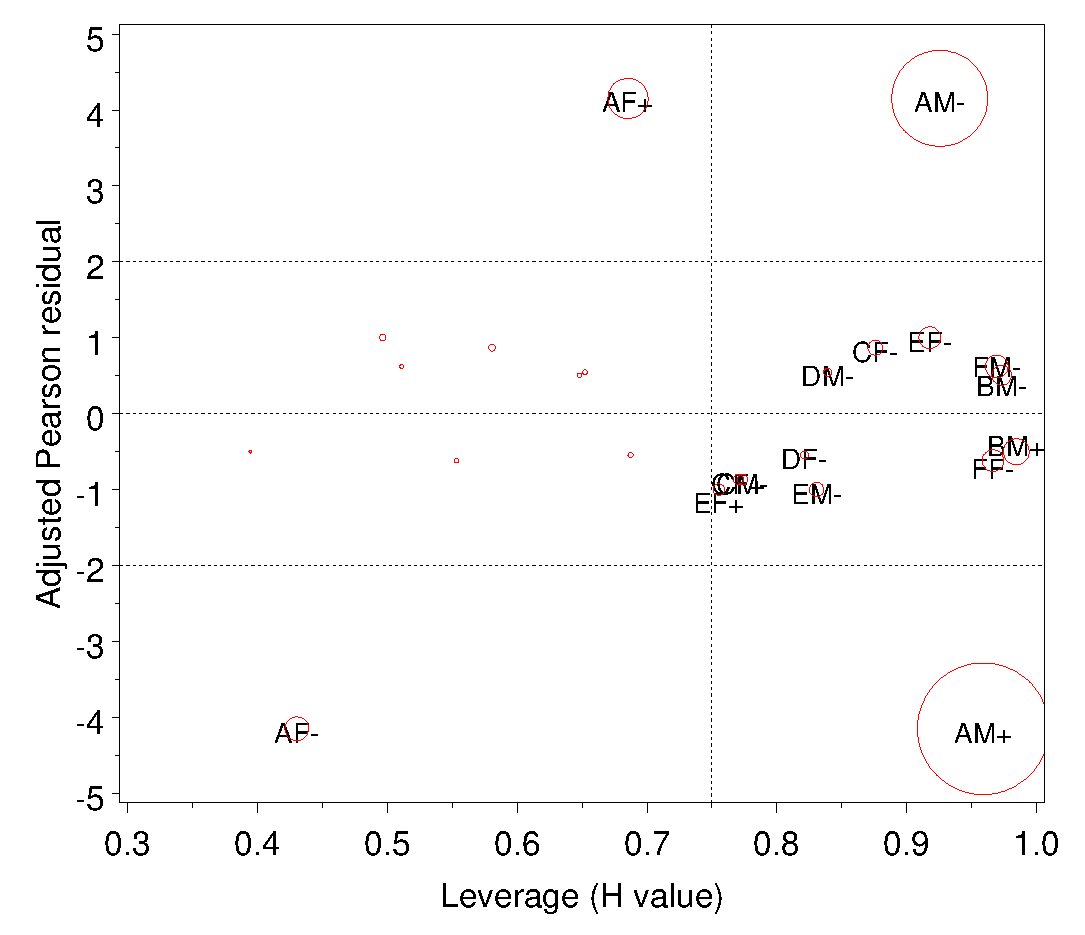
\includegraphics[width=1\linewidth,clip]{fig/genberk11}
 \end{minipage}
 \hfill
 \begin{minipage}[c]{.33\textwidth}
  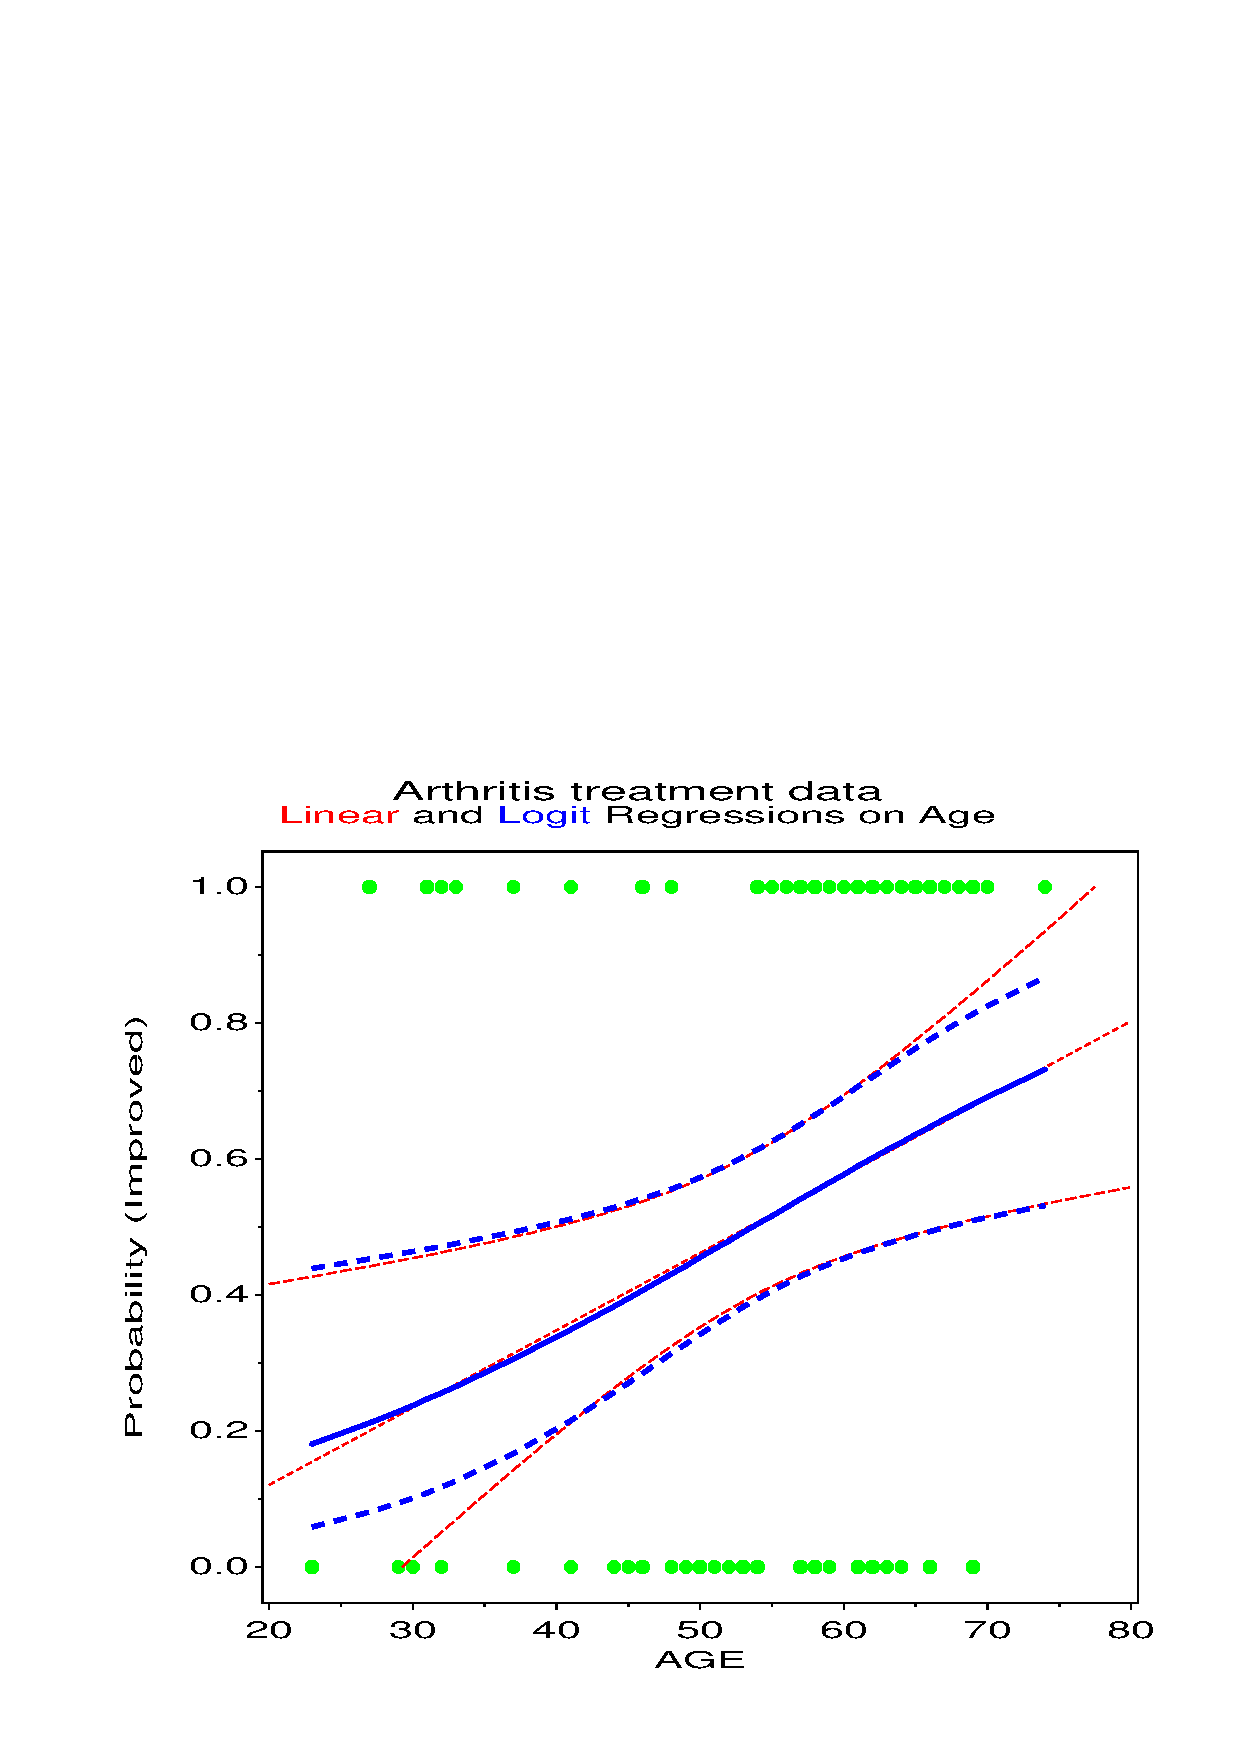
\includegraphics[width=1\linewidth,clip]{fig/logist1c1}
 \end{minipage}

Topics:
  \begin{itemize}
    \item Logit models
	  \begin{itemize*} 
	    \item Plots for logit models
		\item Diagnostic plots for generalized linear models
	  \end{itemize*} 
	\item Logistic regression models
	  \begin{itemize*} 
	    \item Logistic regression: Binary response
		\item Model plots
		\item Effect plots for generalized linear models
		\item Influence measures and diagnostic plots
		\item Polytomous responses
	  \end{itemize*} 
  \end{itemize}
\end{frame}

\section{Logit models}
\section{Logit models}\label{sec:loglin-logit}
Because \loglin\ models are  formulated as models for the
log (expected) frequency, they make no distinction between
response and explanatory variables.
In effect, they treat all variables as responses.
Logit models, on the other hand,
describe how the log odds for one variable depends on other,
explanatory variables.
There is a close connection between the two:
When there is a response variable, each logit model for that response
is equivalent to a \loglin\ model.
This relationship often provides a simpler way to formulate and test
the model, and to plot and interpret the fitted results.
The price paid for this simplicity is that associations among the
explanatory variables are not expressed in the model.

Consider, for example, the model of homogeneous association,
\eqref{eq:lno3way} for a three-way table, and let variable $C$
be a binary response.  Under this model, the logit for variable $C$
is
\begin{eqnarray*}
  L_{ij}  =
  \log \left(  \frac{\pi_{ij|1}}{\pi_{ij|2}} \right) & = &
  \log \left(  \frac{m_{ij1}}{m_{ij2}} \right) \\
    &  = &
  \log (m_{ij1}) - \log (m_{ij2})
  \period
\end{eqnarray*}
Substituting from \eqref{eq:lno3way}, we find that all terms which do not
involve variable $C$ cancel, and we are left with

\begin{eqnarray} \label{eq:logitab1}
  L_{ij}  =
  \log ( m_{ij1} /  m_{ij2} )  & = &
  ( \lambda_1^C - \lambda_2^C )  +
  ( \lambda_{i1}^{AC} - \lambda_{i2}^{AC} )  +
  ( \lambda_{j1}^{BC} - \lambda_{j2}^{BC} )  \nonumber \\
  &  = &
  2 \lambda_1^C   +   2 \lambda_{i1}^{AC} +   2 \lambda_{j1}^{BC}
\end{eqnarray}
because all \(\lambda\) terms sum  to zero.  We are interested in how these
logits depend on $A$ and $B$, so we may replace the $\lambda$ parameters
with new parameters,
 \(\alpha  = 2
\lambda_1^C\), \(\beta _i^A = 2 \lambda_{i1}^{AC}\), etc., which express this relation more directly,
\begin{equation}\label{eq:logitab2}
  L_{ij}  =
  \alpha   +  \beta _i^A +  \beta _j^B
  \period
\end{equation}
In the logit model \eqref{eq:logitab2}, the response, $C$, is affected
by both $A$ and $B$, which have additive effects on the log odds of response
category $C_1$ compared to $C_2$.
The terms $\beta _i^A$ and  $\beta _j^B$
correspond directly to $[AC]$ and $[BC]$ in the \loglin\ model \eqref{eq:lno3way}. The association among the explanatory variables,
$[AB]$ is assumed in the logit model, but this model provides no explicit
representation of that association.  The logit model \eqref{eq:logitab1}
is equivalent to the \loglin\ model $[AB] [AC] [BC]$ in goodness-of-fit
and fitted values, and parameters in the two models correspond directly.

More generally, when there is a binary response variable, say $R$, and
one or more explanatory variables, $A, B, C, \dots$, any logit model
for $R$ has an equivalent \loglin\ form.
Every term in the logit model, such as $\beta_{ik}^{AC}$, corresponds to
an association of those factors with $R$, that is, $[ACR]$ in the
equivalent \loglin\ model.  The \loglin\ model must also include all
associations among the explanatory factors, the term $[A B C \dots]$.
Conversely, any \loglin\ model which includes all associations among
the explanatory variables has an equivalent logit form.
When the response factor has more than two categories, models for
generalized logits have equivalent \loglin\ form.

\begin{Example}[berkeley7]{Berkeley admissions}
The homogeneous association model, $[AD] [AG] [DG]$
did not fit the Berkeley admissions data very well,
and we saw that the term $[AG]$ was unnecessary.
Nevertheless, it is instructive to consider the equivalent logit model.
We illustrate the features of the logit model which lead to the same
conclusions and simplified interpretation from graphical displays.

Because Admission
is a binary response variable, model \eqref{eq:berk1} is equivalent
to the logit model,

\begin{equation}\label{eq:berk3}
  \log \left(
  \frac{m_{ \mbox{\scriptsize{Admit}} (ij) }} {m_{ \mbox{\scriptsize{Reject}} (ij) }}
  \right)
  =
  \alpha   +  \beta _i^{\mbox{\scriptsize Dept}}
  +  \beta _j^{\mbox{\scriptsize Gender}}
  \period
\end{equation}
That is, the logit model \eqref{eq:berk3} asserts that department and
gender have additive effects on the odds of admission.
This model may be fit with \PROC{CATMOD}
as shown below, using the variable \pname{admit} as the response
and \pname{dept} and \pname{gender} as predictors.
The option \pname{order=data} is used so that \PROC{CATMOD} will
form the logit for 'Admitted', the category which appears first
in the \Dset.
The \stmt{RESPONSE}{CATMOD} is used
to create an \ODS\
containing observed and fitted logits, which are graphed
(see \exref{ex:berkeley8}) in
\figref{fig:catberk2}.

\begin{listing}
proc catmod order=data
            data=berkeley;
   weight freq;
   response / out=predict;
   model admit = dept gender / ml noiter noprofile ;
\end{listing}

The model fit statistics and parameter estimates for the model
\eqref{eq:berk3} are shown in \outref{out:catberk2.1}.
Note that the \LR\ \GSQ\ for this model is the same as
that for the \loglin\ model $[AD][AG][DG]$
shown in \outref{out:catberk5.1} and in \outref{out:genberk2.1}
and the Wald \chisq\ values for \pname{dept} and \pname{gender}
in \outref{out:catberk2.1}
are similar to the \chisq\ values for the association of each
of these with \pname{admit}
in the \loglin\ model.

\begin{Output}[htb]
\caption{Berkeley admissions data, fit statistics and parameter estimates for the logit model \eqref{eq:berk3}}\label{out:catberk2.1}
\small
\verbatiminput{ch7/out/catberk2.1}
\end{Output}

As in logistic regression models, parameter estimates may be interpreted
as increments in the log odds, or $\exp(\beta)$ may be interpreted
as the multiple of the odds associated with the explanatory categories.
Because \PROC{CATMOD} uses zero-sum constraints,
$\sum \beta_i^{\mbox{\scriptsize   Dept}} =0$ and
$\sum \beta_j^{\mbox{\scriptsize   Gender}} =0$, the parameters for the
last level of any factor
is found as the negative of the sum of the parameters listed.

Thus, $\beta_1^{\mbox{\scriptsize   Gender}} = -0.0499$
is the increment to the log odds of admission for men,%
\footnote{$\beta_1^{\mbox{\scriptsize   Gender}}$ refers to
the first level of \pname{gender} to appear in the \pname{berkeley}
\Dset, because \pname{order=data} was used on the \PROC{CATMOD} statement.}
and therefore $\beta_2^{\mbox{\scriptsize Gender}} = +0.0499$ for women.
Overall, but controlling for department, women were $\exp(2 \times 0.0499) = 1.105$
times as likely to be admitted to graduate school than male applicants
in 1973.
The logit parameters for \pname{dept} in \outref{out:catberk2.1} decrease
over departments A--E; the value for department F is $-(1.274 + 1.231 + \cdots
-0.465) = -2.032$.
These values correspond to the decline in the fitted logits
over department seen in \figref{fig:catberk2}.

Logit models are easier to interpret than the corresponding \loglin\
models because there are fewer parameters,
and because these parameters pertain to the odds of a response category
rather than to cell frequency.
Nevertheless, interpretation is often easier still from a graph than from the
parameter values.
\end{Example}


\subsection{Plotting results for logit models}

Logit models may also be interpreted through plots of observed and
fitted values, either in terms of the logit for one response category
or in terms of the equivalent response probability.
Plots of log odds generally have a simpler, additive form, such as
the parallel curves in \figref{fig:catberk2},
but the effects may be easier to understand in terms of
probabilities.
As with logistic regression models, both goals may often be
achieved by plotting on the logit scale and adding a second vertical
axis showing the corresponding probabilities.
These plots are similar to those described in \secref{sec:logist-quant}
and \secref{sec:logist-qual}, but the plotting steps differ because
the output information from \PROC{CATMOD} is structured differently
from that provided by \PROC{LOGISTIC}.

Such plots are facilitated by the \macro{CATPLOT} (\macref{mac:catplot}).
The macro uses the \ODS\  produced with the \pname{OUT=} option on the \stmt{RESPONSE}{CATMOD}.
This \Dset\ normally contains both logit values
and probability values, and either type may be plotted, with observed
and fitted values, and optional confidence intervals.
A utility macro, \pname{PSCALE} (\macref{mac:pscale}) may be used to add a probability scale
to a plot of log odds.
\begin{Example}[berkeley8]{Berkeley admissions}
The \ODS\ \pname{predict} from the logit model, \pname{admit = dept gender},
for the Berkeley data is shown partially in \outref{out:catberk2.2}.
Each of the $ 2 \times 6$ samples defined by the explanatory factors
\pname{dept, gender}
gives rise to three observations: two response probabilities and
one logit, distinguished by the variable \verb|_TYPE_|.
\begin{Output}[htb]
\caption{Output \Dset\ \pname{predict} from the logit model for Berkeley admissions (partial)}\label{out:catberk2.2}
\small
\verbatiminput{ch7/out/catberk2.2}
\end{Output}

%% one figure
\begin{figure}[htb]
  \centering
  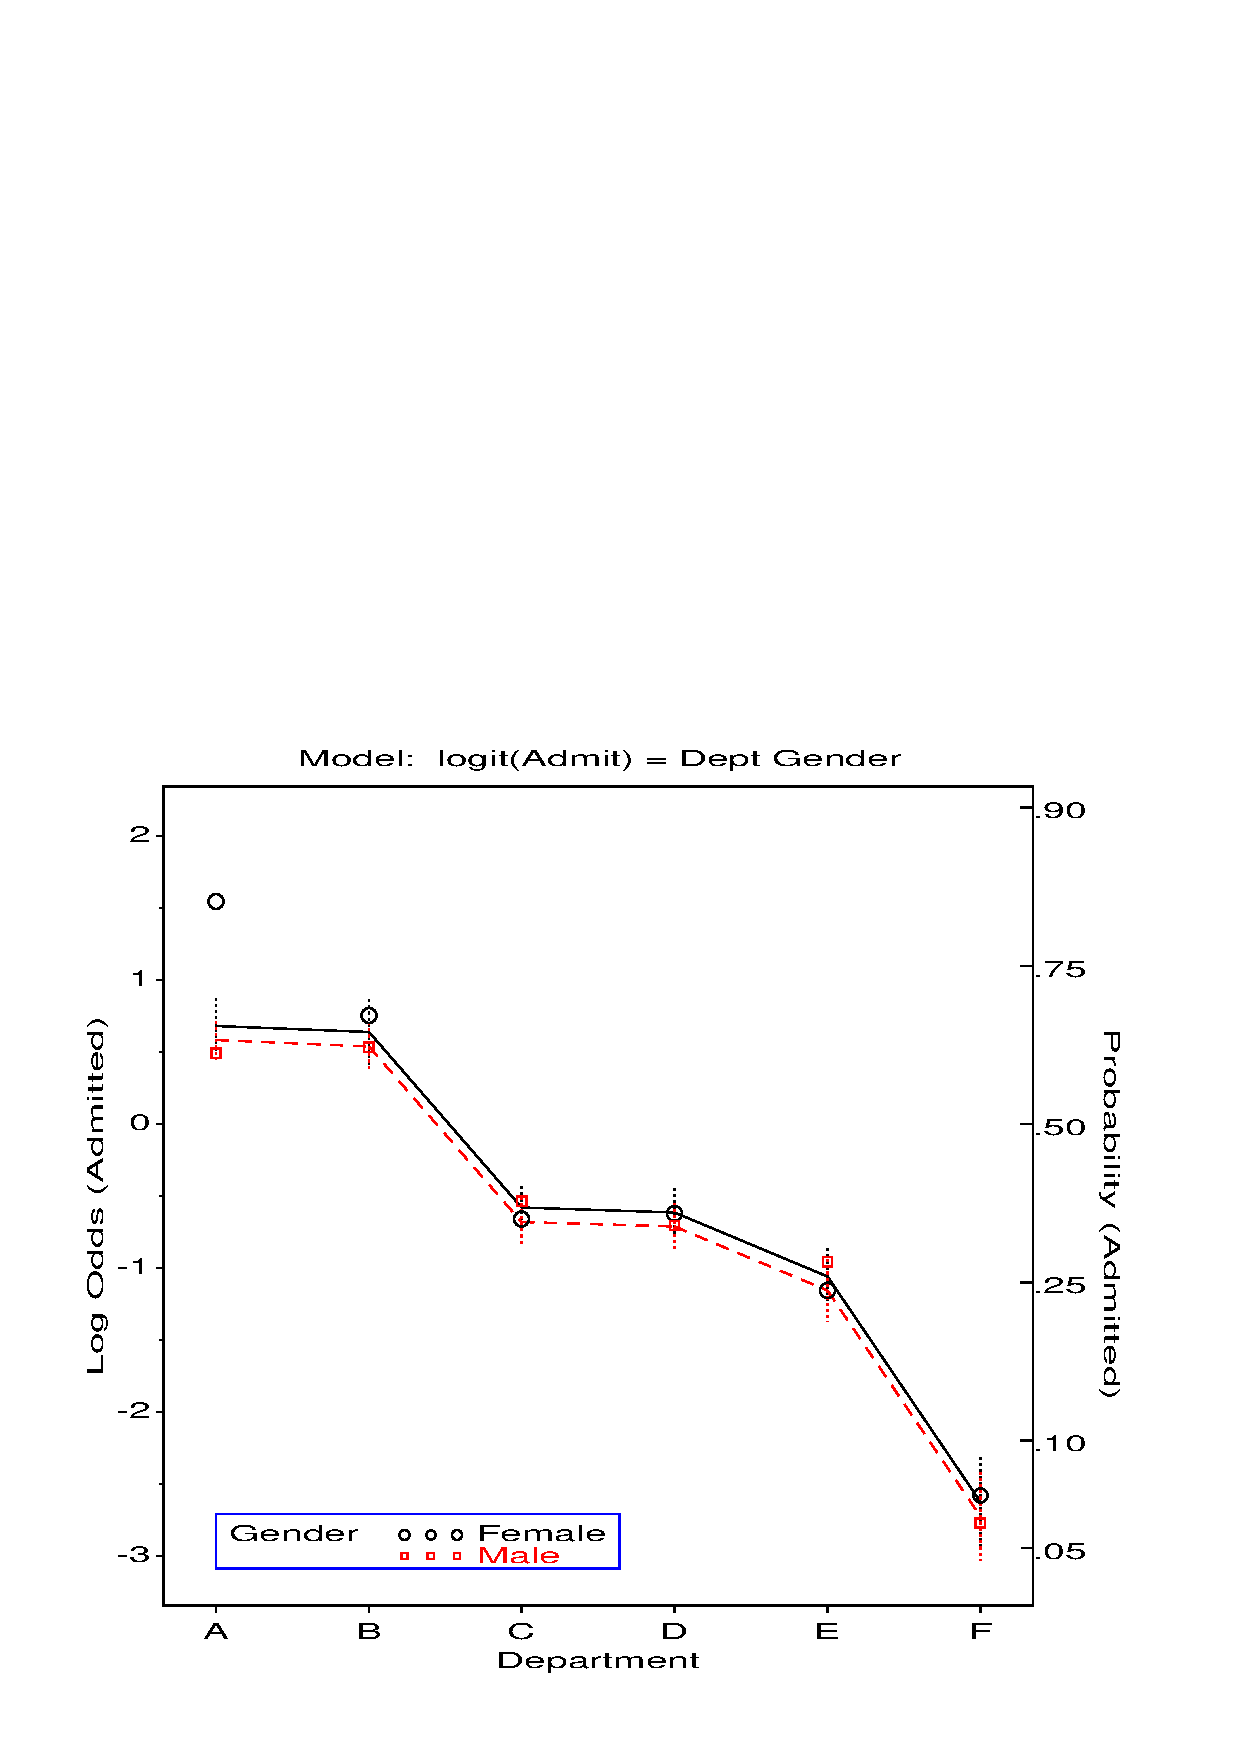
\includegraphics[scale=.6]{catberk2}
  \caption[Observed and fitted log odds of admission in the logit model]{Observed (points) and fitted (lines) log odds of admission in the logit model
  corresponding to [AD][AG][DG].  The error bars show individual 95\%
  confidence intervals around each fitted logit.}%
  \label{fig:catberk2}
\end{figure}

The statements below draw the plot of observed and predicted logits
(\verb|_type_='FUNCTION'|) shown in \figref{fig:catberk2}.
The \macro{PSCALE} constructs an \ADS\
which draws the probability values on the right vertical axis in the
plot.
The label for this axis is specified in the \stmt{TITLE}{GPLOT}, with
an angle, \pname{A=-90}, meaning the right-hand side, rotated \degree{90}.
By default, the macro uses the \pname{AXIS} and \pname{SYMBOL}
statements defined before the macro call.
Separate curves are
drawn for each level of the \pname{CLASS=GENDER} variable.
The values of the \pname{CLASS} variable may be labeled in the plot
or supplied in a \stmt{LEGEND}{CATPLOT}.
The parameter \pname{Z=1.96} specifies the multiple of
the standard error of the fitted logit (\verb|_SEPRED_|) used to
draw the error bars in the plot,
giving (asymptotic) 95\% individual confidence intervals.
\begin{listing}
%pscale(lo=-4, hi=3, anno=pscale, prob=%str(0.05,.1,.25,.5,.75,.9));

title h=1.6 'Model:  logit(Admit) = Dept Gender'
            a=-90 'Probability (Admitted)'
      h=3.5 a=-90 ' ';
legend1 position=(bottom inside left)  offset=(4,3)
        mode=share cborder=blue across=1
        shape=symbol(6,1.5) label=('Gender')
        value=(c=black 'Female'
               c=red   'Male');
axis1 order=(-3 to 2) offset=(4)
      label=(a=90 'Log Odds (Admitted)');
axis2 label=('Department') offset=(4);
symbol1 i=none v=circle h=1.7 c=black;
symbol2 i=none v=dot    h=1.7 c=red  ;
%catplot(data=predict,
   xc=dept, y=_obs_, class=gender,
   type=FUNCTION,
   z=1.96, anno=pscale, legend=legend1);
\end{listing}

The effects seen in our earlier analyses (Examples~\ref{ex:berkeley4}
and \ref{ex:berkeley4b})
may all be observed in this
plot.
The effect of gender is shown by the constant separation
between the two curves.
From the plot we see that this effect is very small and nonsignificant (compared
with the error bars).
If the gender effect were omitted from the model,
the fitted logits would be the same
for men and women applying to each department, and would plot as a curve
parallel to, but in between, the two shown in the graph.
Most of the observed points are quite close to their predicted values,
except in Department A,
where the probability of admittance for women is substantially
greater than that for men.
In \exref{ex:berkeley6} we dealt with this by allowing one extra parameter
for an association between admission and gender in department A,
giving the \loglin\ model \eqref{eq:berk2}.

We can see what this model ``looks like'' by recasting it in logit form.
The \loglin\ model \eqref{eq:berk2}
has an equivalent logit formulation, which also adds a 1 df term for an
effect of gender in department A,
\begin{equation}\label{eq:berk4}
  L_{ij} =
  \alpha   +  \beta _i^{\mbox{\scriptsize Dept}}
  +  \delta_{j=1} \beta^{\mbox{\scriptsize Gender}}
  \period
\end{equation}

This model may be fit
with \PROC{CATMOD} as shown below.  The association term between admission
and gender for Dept. A (\texttt{dept1AG}) is fit as a \pname{DIRECT}
variable.  The \pname{gender} variable is not included in the
\stmt{MODEL}{CATMOD}, so it must be listed in the
\stmt{POPULATION}{CATMOD}.
Because the \macro{CATPLOT}
uses the values in the \ODS, the plotting step is unchanged.

\begin{listing}
data berkeley;
   set berkeley;
   dept1AG = (gender='F') * (dept=1);

proc catmod order=data
            data=berkeley;
   weight freq;
   population dept gender;
   direct dept1AG;
   response / out=predict;
   model admit = dept dept1AG / ml noiter noprofile ;
%catplot(data=predict, xc=dept, class=gender, type=FUNCTION,
   z=1.96, legend=legend1);
\end{listing}

%% one figure
\begin{figure}[htb]
  \centering
  \includegraphics[scale=.6]{catberk6}
  \caption{Observed and fitted logits for model \eqref{eq:berk2}}%
  \label{fig:catberk6}
\end{figure}
The resulting plot for this model is shown in \figref{fig:catberk6}.
The graph gives a visual interpretation of the model
\eqref{eq:berk2} and its logit form, \eqref{eq:berk4}:
No effect of gender on admission, except in department A, where the
extra parameter allows perfect fit.
\end{Example}


\subsection{Zero frequencies}
Cells with frequencies of zero create problems for \loglin\ and logit
models.  For \loglin\ models, most of the derivations of expected
frequencies and other quantities assume $n_{ijk\cdots} > 0$.
In logit models, the observed log odds (e.g., for a three-way table),
$\log ( n_{ij1} / n_{ij2} )$, will be undefined if either frequency is
zero.

Zero frequencies may occur in \ctabs\ for two different reasons:
\begin{description}
\item[structural zeros] (also called \emph{fixed zeros}) will occur when it is impossible to observe
values for some combinations of the variables.
For example, suppose we have three different methods of contacting
people at risk for some obscure genetically inherited disease:
newspaper advertisement, telephone campaign, and radio appeal.
If each person contacted in any way is classified dichotomously
by the three methods of contact, there can never be a non-zero
frequency in the `No-No-No' cell.%
\footnote{Yet, if we fit an unsaturated model, expected frequencies
may be estimated for all cells, and provide a means to estimate
the total number at risk in the population.
See \citet[Section 5.4]{Lindsey:95}.}
\item[sampling zeros] (also called \emph{random zeros})
occur when the total size of the sample is not large enough in relation to the probabilities in each of the cells to assure that someone will be observed
in every cell.
For example, in a European survey of religious affiliation and occupation,
we may not happen to observe any Muslim vineyard-workers in France, although such individuals surely exist.
Even when zero frequencies do not occur, tables with many cells relative to
the total frequency tend to produce small expected frequencies in at
least some cells, which tends to make  the \chisq\ statistics for model fit
and Wald statistics for individual terms unreliable.
\end{description}

\PROC{CATMOD} takes a simple approach to distinguishing these two cases:
Cells with zero frequency are simply deleted from the \ctab,
and thus are treated as structural zeros.  To avoid this, some corrective
action is needed.
One solution (for sampling zeros) is to collapse categories of some variables,
but we are often loath to do this for fear of loss of information.

Other suggestions are:
\begin{seriate}
\item Add a small positive quantity (0.5 is usually recommended) to every
cell in the \ctab\ \citep{Goodman:70}, as is done in calculating
empirical log odds (\secref{sec:logist-logodds});
\PROC{CATMOD} provides the \opt{ADDCELL}{CATMOD} in the \stmt{MODEL}{CATMOD} for this purpose,
but this option is ignored for maximum likelihood estimation.
\item Replace sampling zeros by some small number, typically
$10^{-10}$ or smaller \citep{Agresti:90}.
\item Add a small quantity, like 0.1, to all zero cells
\citep{EversNamboodiri:77}.
\end{seriate}

\begin{Example}[reagan]{Race and politics in the 1980 US Presidential vote}
\tabref{tab:reagtab} shows data (\citet[Table 4.12]{Agresti:90}, from \citet{CloggShockey:88})
from the 1982 General Social Survey on
votes in the 1980 US Presidential election for Reagan or for Carter
or other in relation to race and conservatism (1=most liberal,
7=most conservative).
The \Dset\ \pname{vote}, containing the
variables \pname{race}, \pname{cons}, \pname{votefor}, and
\pname{count} is listed in \datref{dat:vote}.

\begin{table}[htb]
 \caption{1982 General Social Survey: Reagan vs. Carter, by Race and Conservatism}\label{tab:reagtab}
 \begin{center}
 \begin{tabular}{c rr rr}
  \hline
       & \multicolumn{4}{c}{Race} \\
  Political & \multicolumn{2}{c}{White} & \multicolumn{2}{c}{Non White} \\ 
  \cline{2-5}
  Conservatism & Reagan & Carter/other  & Reagan & Carter/other \\ 
  \hline
  1 & 1 & 12 & 0 & 6 \\ 
  2 & 13 & 57 & 0 & 16 \\ 
  3 & 44 & 71 & 2 & 23 \\ 
  4 & 155 & 146 & 1 & 31 \\ 
  5 & 92 & 61 & 0 & 8 \\ 
  6 & 100 & 41 & 2 & 7 \\ 
  7 & 18 & 8 & 0 & 4 \\ 
  \hline
 \end{tabular}
 \end{center}
\end{table}


It is natural to treat vote for Reagan vs. (Carter or other) as the response,
and race and conservatism as predictors in this $2 \times 2 \times 7$
table, with variables VoteFor ($V$), Race ($R$) and Conservatism ($C$).
Before fitting models, it is useful to take an exploratory look
at the data.
The fourfold display shown in \figref{fig:reagan1a}
shows separate panels for each level of conservatism.
In order to focus on the tendency to vote for Reagan vs.\ (Carter or other)
among Whites compared to Non Whites,
the number of White and Non White respondents were equated in each
panel in this figure.
With this standardization confidence rings will overlap in the left
and right quadrants ( Reagan vs.\ Carter or other) when the (conditional)
odds ratio
does not differ significantly from 1.

%% one figure
\begin{figure}[htb]
  \centering
  \includegraphics[width=\textwidth,clip]{reagan1a}
  \caption[Fourfold display for Vote, by Race and Conservatism]{Fourfold display for Vote, by Race and Conservatism, equating the number of White and Non White respondents at each level of Conservatism}%
  \label{fig:reagan1a}
\end{figure}

Thus, among Whites, in the bottom half of each panel,
we may compare the areas of the left and right quadrants,
and see that the propensity to vote for Reagan increases with
conservatism.
A similar trend is evident among Non White respondents, but there
are a number of zero frequencies here, among Non Whites who indicated they
voted for Reagan.

The conditional odds ratios for Vote and Race given Conservatism are all in the same direction, indicating that Whites were more likely to vote for
Reagan at \emph{any} level of Conservatism.
The \sasprog{fourfold}  gives the test of homogeneity of odds ratios
shown in \outref{out:reagan1.1},
which is equivalent to a test for lack-of-fit of the
homogeneous association \loglin\ model $[RC] [VR] [VC]$.
The tests of conditional independence, $V \perp R \given C$,
suggest that voting preference depends on race, and possibly conservatism.

\ixon{zero cells}
To illustrate the problem of zero cells, consider tests of fit of the
saturated model, $[RCV]$, and of the homogeneous association model,
$[RC] [VR] [VC]$, fit as \loglin\ models under three conditions:
\begin{seriate}
\item no adjustment for zeros,
\item replace zeros by $10^{-10}$, and
\item add 0.5 to each cell.
\end{seriate}
In each case, the models are fit
with the statements below, after possible adjustment to the \pname{count}
variable.
The results are summarized in \tabref{tab:reagzero}.
\begin{listing}
proc catmod data=vote;
   weight count;
   model cons*race*votefor = _response_ / ml noiter noresponse noprofile;
   loglin cons|race|votefor / title='Saturated model';
  run;
   loglin cons|race|votefor @2 / title='No 3-way association';
\end{listing}
In case (a), the four zero cell are treated as structural zeros, and
deleted, leaving only 2 df for the test of lack-of-fit in the
no-3-way model.
In case (b), the main effect parameter for Race cannot be estimated
and there is, paradoxically, 1 df for the test of the saturated model.
Case (c), adding 0.5 to each cell, has no anomalies, and we adopt this
solution for this example. In other cases it is recommended to compare
several approaches to determine if any conclusions are affected by
the presence of zero cells.
\ix{zeros!structural}

\begin{table}[htb]
 \caption{Effects of zero-cell actions on \loglin\ models for \pname{vote} data}\label{tab:reagzero}
 \begin{center}
 \begin{tabular}{l rrrr}
  \hline
   \multicolumn{1}{r}{Model:}  & \multicolumn{2}{c}{$[RCV]$} & \multicolumn{2}{c}{$[RC] [VR] [VC]$} \\
  Action                     & df & \GSQ\ & df & \GSQ\ \\ 
  \hline
(a)  None                       & 0 & . & 2 & 1.89 \\ 
(b)  $n=0 \rightarrow 10^{-10}$ & 1 & 0.00 & 6 & 4.96 \\ 
(c)  $n	\rightarrow n+\frac12$ & 0 & . & 6 & 3.45 \\ 
  \hline
 \end{tabular}
 \end{center}
\end{table}

\ixoff{zero cells}

\begin{Output}[htb]
\caption{Vote data: Test of Homogeneity of odds ratios}\label{out:reagan1.1}
\small
\verbatiminput{ch7/out/reagan1.1}
\end{Output}

We proceed to fit a main effects logit model.
Treating the vote for Reagan vs. Carter or other as the response, the
logit model with nominal main effects for race and conservatism is

\begin{equation} \label{eq:logrnom}
    \logit ( \mbox{Reagan} / \mbox{Carter} )  =
    \alpha   +
    \beta _i^{\mbox{\scriptsize Race}}  +
    \beta _j^{\mbox{\scriptsize Cons}}
	 \period
\end{equation}
Model \eqref{eq:logrnom} may be fit with \PROC{CATMOD} as follows. \begin{listing}
data vote;
    set vote;
    count = count + 0.5;
proc catmod data=vote order=data;
   weight count;
   response / out=predict;
   model votefor = race cons / noiter noresponse noprofile;
\end{listing}

The model fit statistics and parameter estimates for the logit model
\eqref{eq:logrnom} are shown in \outref{out:glogit1.1}.
The model fits quite well.
\begin{Output}[htb]
\caption{Vote data: Fit of the nominal main effects model}\label{out:glogit1.1}
\small
\verbatiminput{ch7/out/glogit1.1}
\end{Output}

To interpret the model, we plot the observed and predicted logits, with
90\% confidence intervals, as shown below.  The \macro{CATPLOT}
gives \figref{fig:glogit11}.
\begin{listing}
%pscale(lo=-5, hi=2.3, anno=pscale, prob=%str(0.01,.05,.1,.25,.5,.75,.9));

axis1 order=(-5 to 2) offset=(0,3)
      label=(a=90 'Logit (Reagan / Carter)');
axis2 label=('Conservatism') offset=(2);
symbol1 i=none v=circle h=1.9 c=black;
symbol2 i=none v=square h=1.7 c=red  ;
legend1 position=(bottom inside center) offset=(,2);
%catplot(data=predict, class=race, x=cons, z=1.65, anno=pscale,
   legend=legend1);
\end{listing}

%% one figure
\begin{figure}[htb]
  \centering
  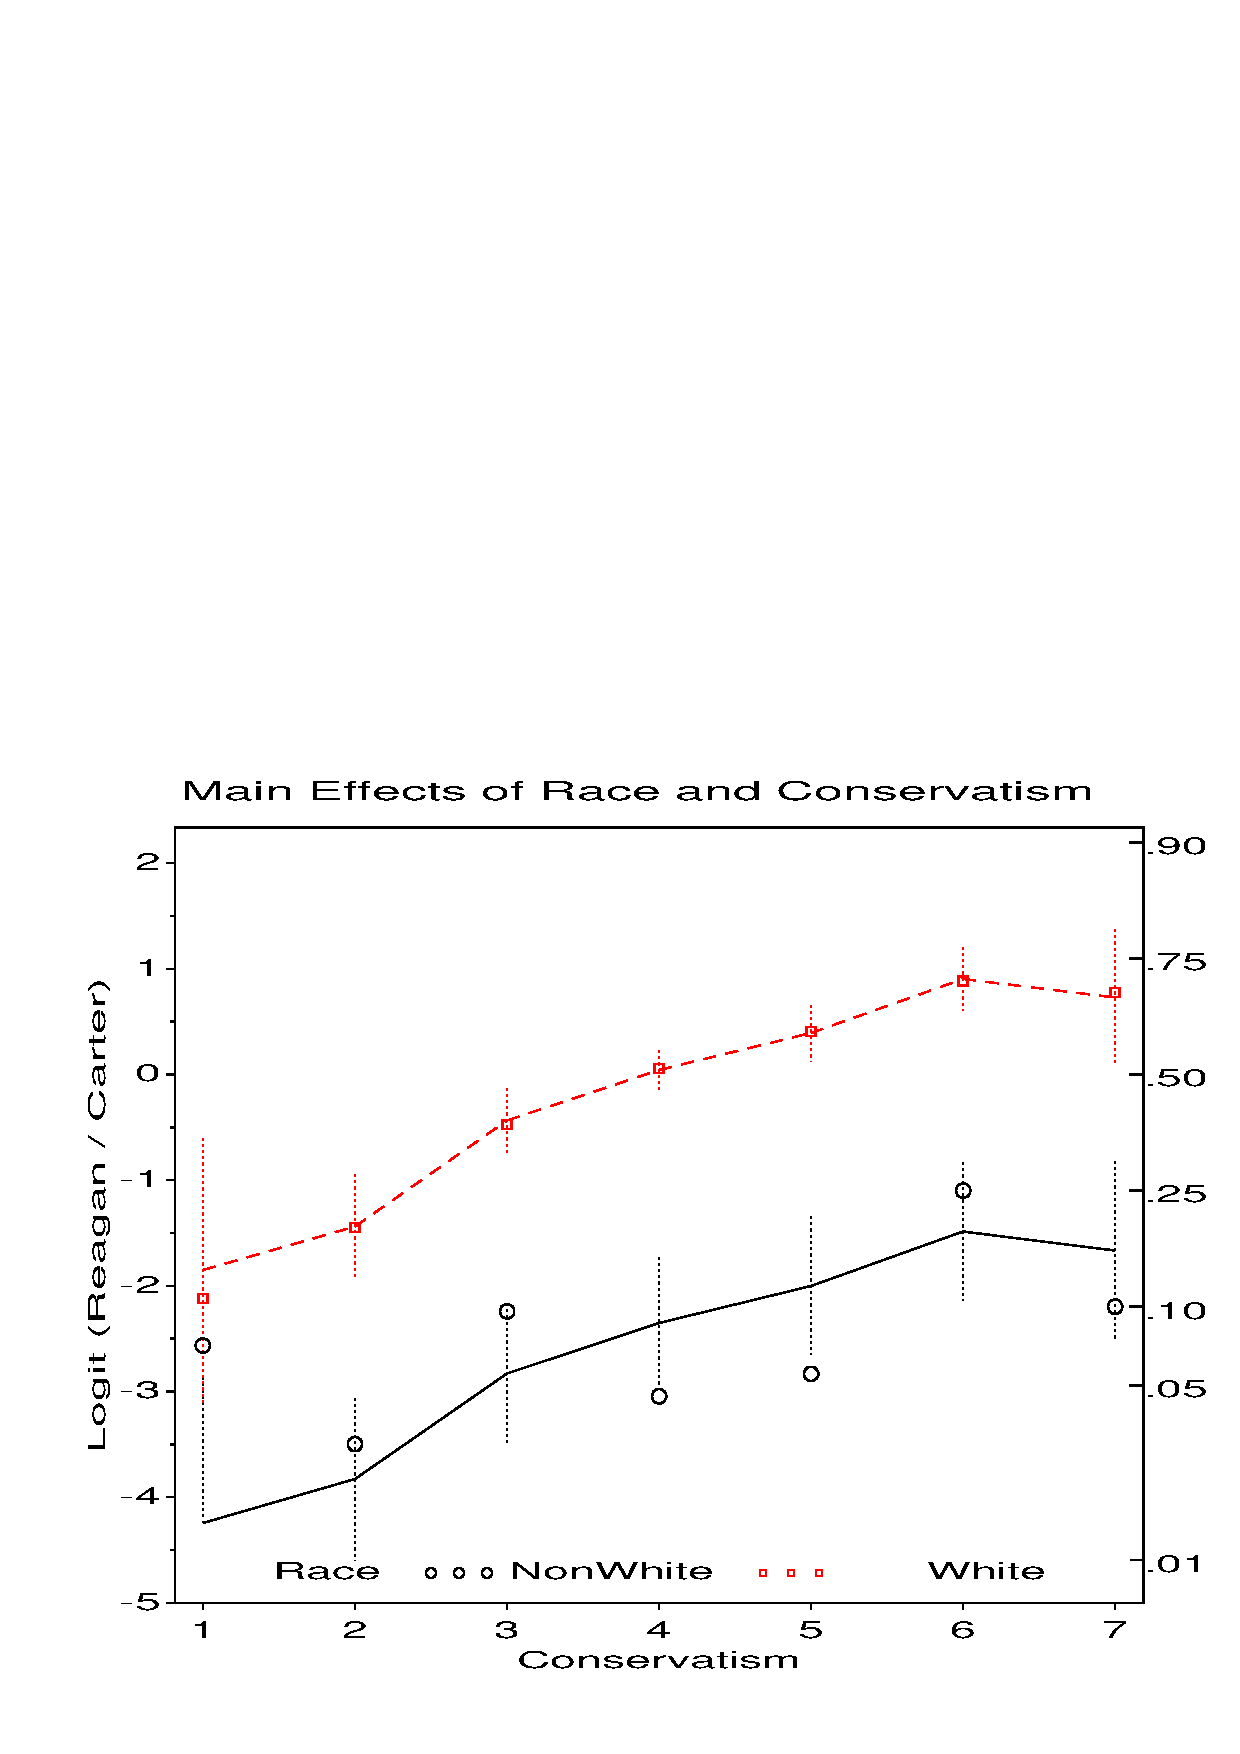
\includegraphics[scale=.6]{glogit11}
  \caption[Observed and fitted logits for main effects model]{Observed (points) and fitted (lines) logits for main effects model.  Dotted lines show a 90\% confidence interval around the predicted log odds.}%
  \label{fig:glogit11}
\end{figure}
Notice that for both Whites and Non Whites, the log odds of voting for
Reagan increases with conservatism.  This is also reflected in the
parameter estimates for \pname{cons} in \outref{out:glogit1.1},
which increase in approximately equal steps.
Model \eqref{eq:logrnom} does not use the ordinal nature of conservatism.
A model which uses conservatism as a direct,
quantitative independent variable ($c$) can be expressed as

\begin{equation} \label{eq:logrlin}
  \mbox{logit ( Reagan / Carter )}  =
  \alpha   +
  \beta _i^{\mbox{\scriptsize Race}}  +
  \beta ^{\mbox{\scriptsize Cons}} \,  c
\end{equation}
Note that there is just one parameter for conservatism,
$ \beta ^{\mbox{\scriptsize Cons}}$, which is interpreted as
an increase in the log odds of a vote for Reagan for each
change of 1 unit in conservatism.
Model \eqref{eq:logrlin} may be fit with \PROC{CATMOD}
just by adding the statement \pname{DIRECT CONS;}
\begin{listing}
proc catmod data=vote order=data;
   direct cons;
   weight count;
   response / out=predict;
   model votefor = race cons / noiter noresponse noprofile ;
   title 'Linear Effect for Conservatism' h=2.5 a=-90 ' ';
\end{listing}
The \LR\ \GSQ\ for this model is $\GSQ (11) = 9.58$, and
the difference in \GSQ\ for Models
\eqref{eq:logrlin} and \eqref{eq:logrnom} is
$\Delta \GSQ (5) = 6.13$,
so the linear model cannot be rejected, given that the nominal
model fits.  The estimate $\widehat{\beta} ^{\mbox{\scriptsize Cons}} = 0.472$
indicates that the odds of voting for Reagan increase by a factor of
$\exp(0.472) = 1.60$ (60\%) for each step of increasing conservatism.

%\begin{Output}[htb]
%\caption{}\label{out:glogit1.2}
%\small
%\verbatiminput{ch7/out/glogit1.2}
%\end{Output}

The observed and fitted logits are plotted exactly as before, using
the same \macro{CATPLOT} call with the new \ODS\ \pname{predict}.
The plot is shown in \figref{fig:glogit12}.
Note that the 90\% confidence limits around predicted values are
noticeably smaller than in \figref{fig:glogit11}.
This is but one advantage of models for ordinal variable,
which we discuss in the following section.
%% one figure
\begin{figure}[htb]
  \centering
  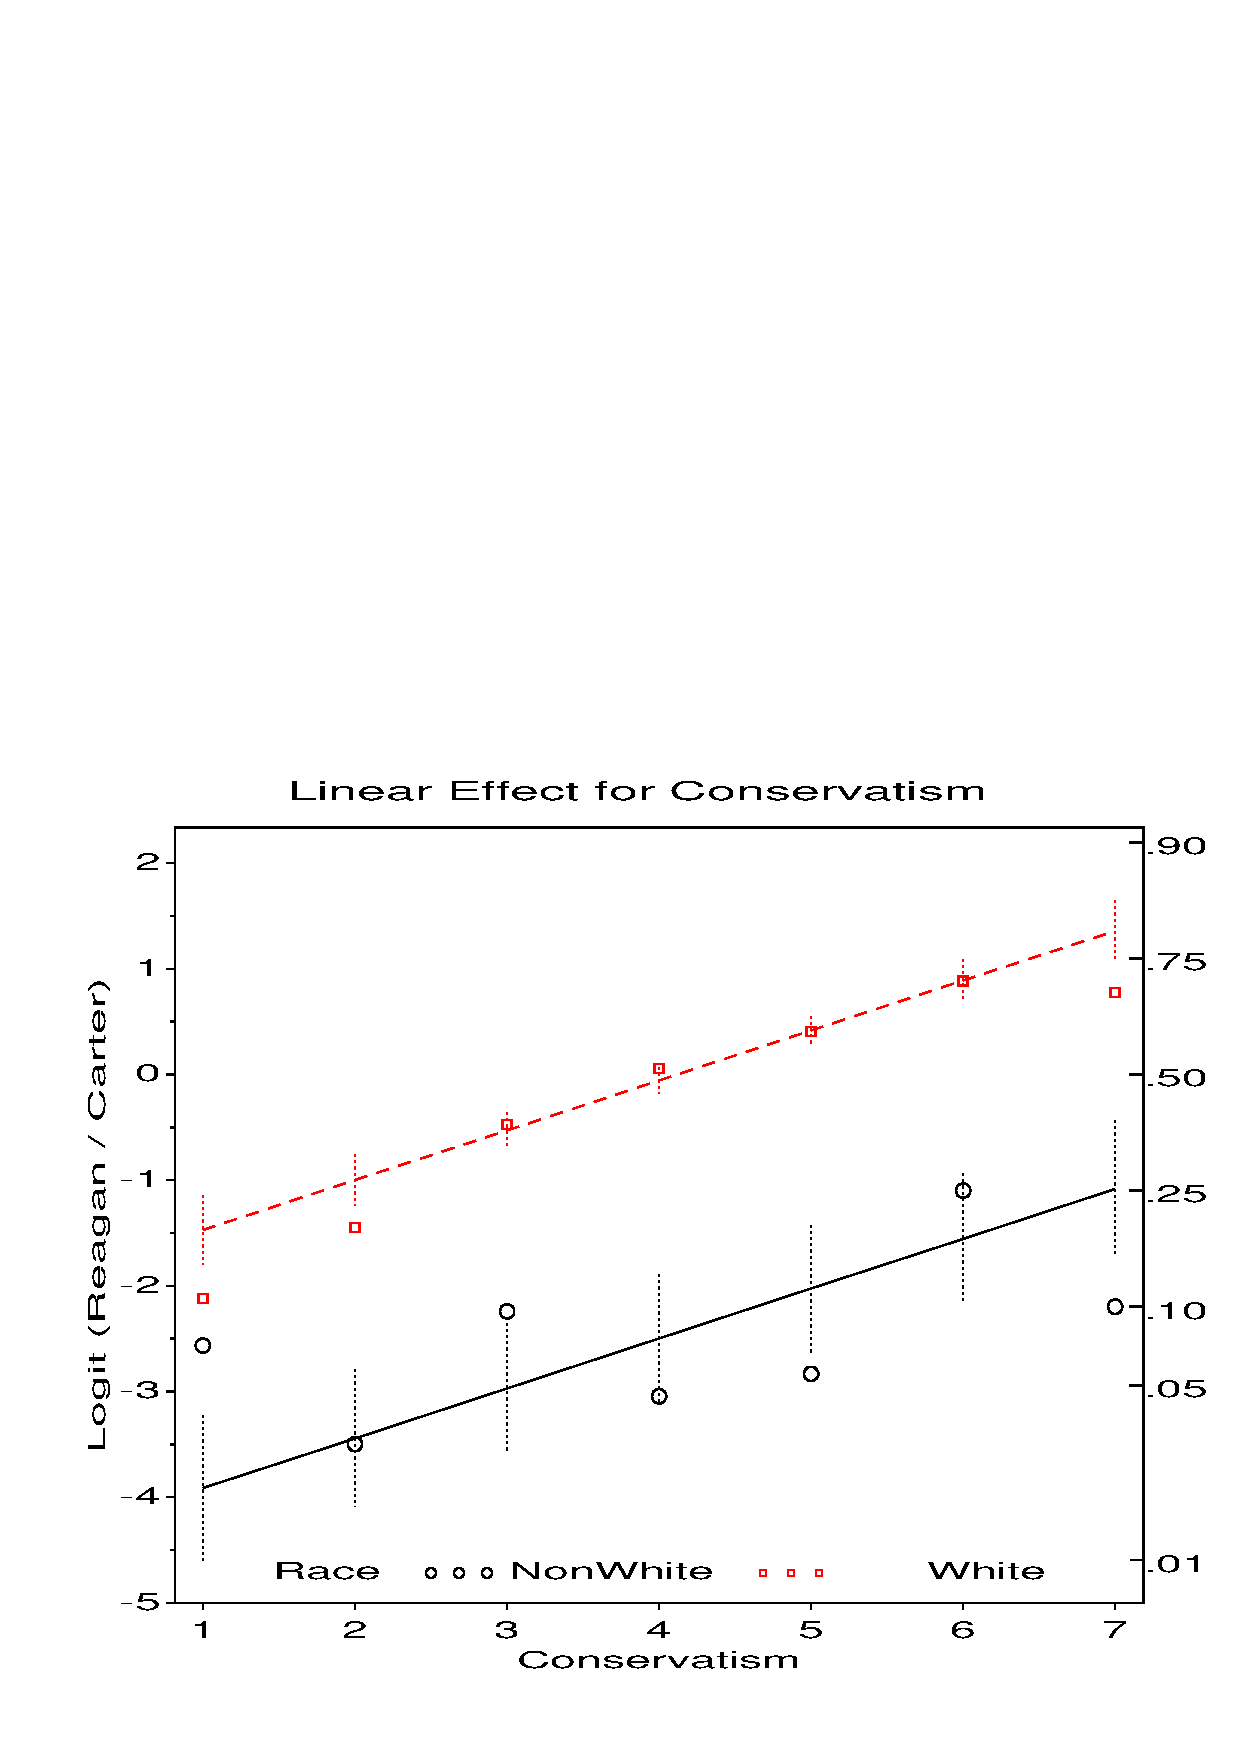
\includegraphics[scale=.6]{glogit12}
  \caption[Observed and fitted logits for linear effect of conservatism]{Observed (points) and fitted (lines) logits for linear effect of conservatism.  Dotted lines show a 90\% confidence interval around the predicted log odds.}%
  \label{fig:glogit12}
\end{figure}
\end{Example}


\section{Logistic regression models}
\renewcommand{\FileName}{logistic1}
\begin{frame}
  \frametitle{Logistic regression models}
  \begin{block}{\large\bfseries Response variable}<1->
      \begin{itemize*}
	   \item Binary response: success/failure, vote: yes/no
	   \item Binomial data: $x$ successes in $n$ trials (grouped data)
	   \item Ordinal response: none < some < severe depression
	   \item Polytomous response: vote Liberal, Tory, NDP, Green
      \end{itemize*}
  \end{block}
  \begin{block}{\large\bfseries Explanatory variables}<2->
      \begin{itemize*}
	  \item Quantitative regressors: age, dose
	  \item Transformed regressors: $\sqrt{\mathrm{age}}$, log(dose)
	  \item Polynomial regressors: age$^2$, age$^3$, $\cdots$
	  \item Categorical predictors: treatment, sex
	  \item Interaction regessors: treatment $\times$ age, sex $\times$ age
	  \end{itemize*}
  \end{block}
\end{frame}

\subsection{Binary response}
\begin{frame}
  \frametitle{Logistic regression models: Binary response}
  \begin{itemize*}
	\item For a binary response, $Y \in (0,1)$, want to predict $\pi = \Pr(Y=1 \given x)$
	\item Linear regression will give predicted values outside $0 \le \pi \le 1$
	\item Logistic model:
	\begin{itemize*}
	  \item $\logit ( \pi_{i}) \equiv \log [ \pi / (1 - \pi)]$ avoids this problem
	  \item logit is interpretable as ``log odds'' that $Y=1$
	\end{itemize*}
	
	\item Probit (normal transform) model $\rightarrow$ similar predictions, but is less
	interpretable
 \begin{center}
  \includegraphics[width=.4\dispwidth,clip]{fig/logitfn}
 \end{center}
  \end{itemize*}

\end{frame}

\begin{frame}
  \frametitle{Logistic regression models: Binary response}
Quantitative predictor: Linear and Logit regression on age
  \begin{itemize*}
	\item Except in extremes, linear
and logistic models give similar predicted values
	\end{itemize*}
\begin{center}
   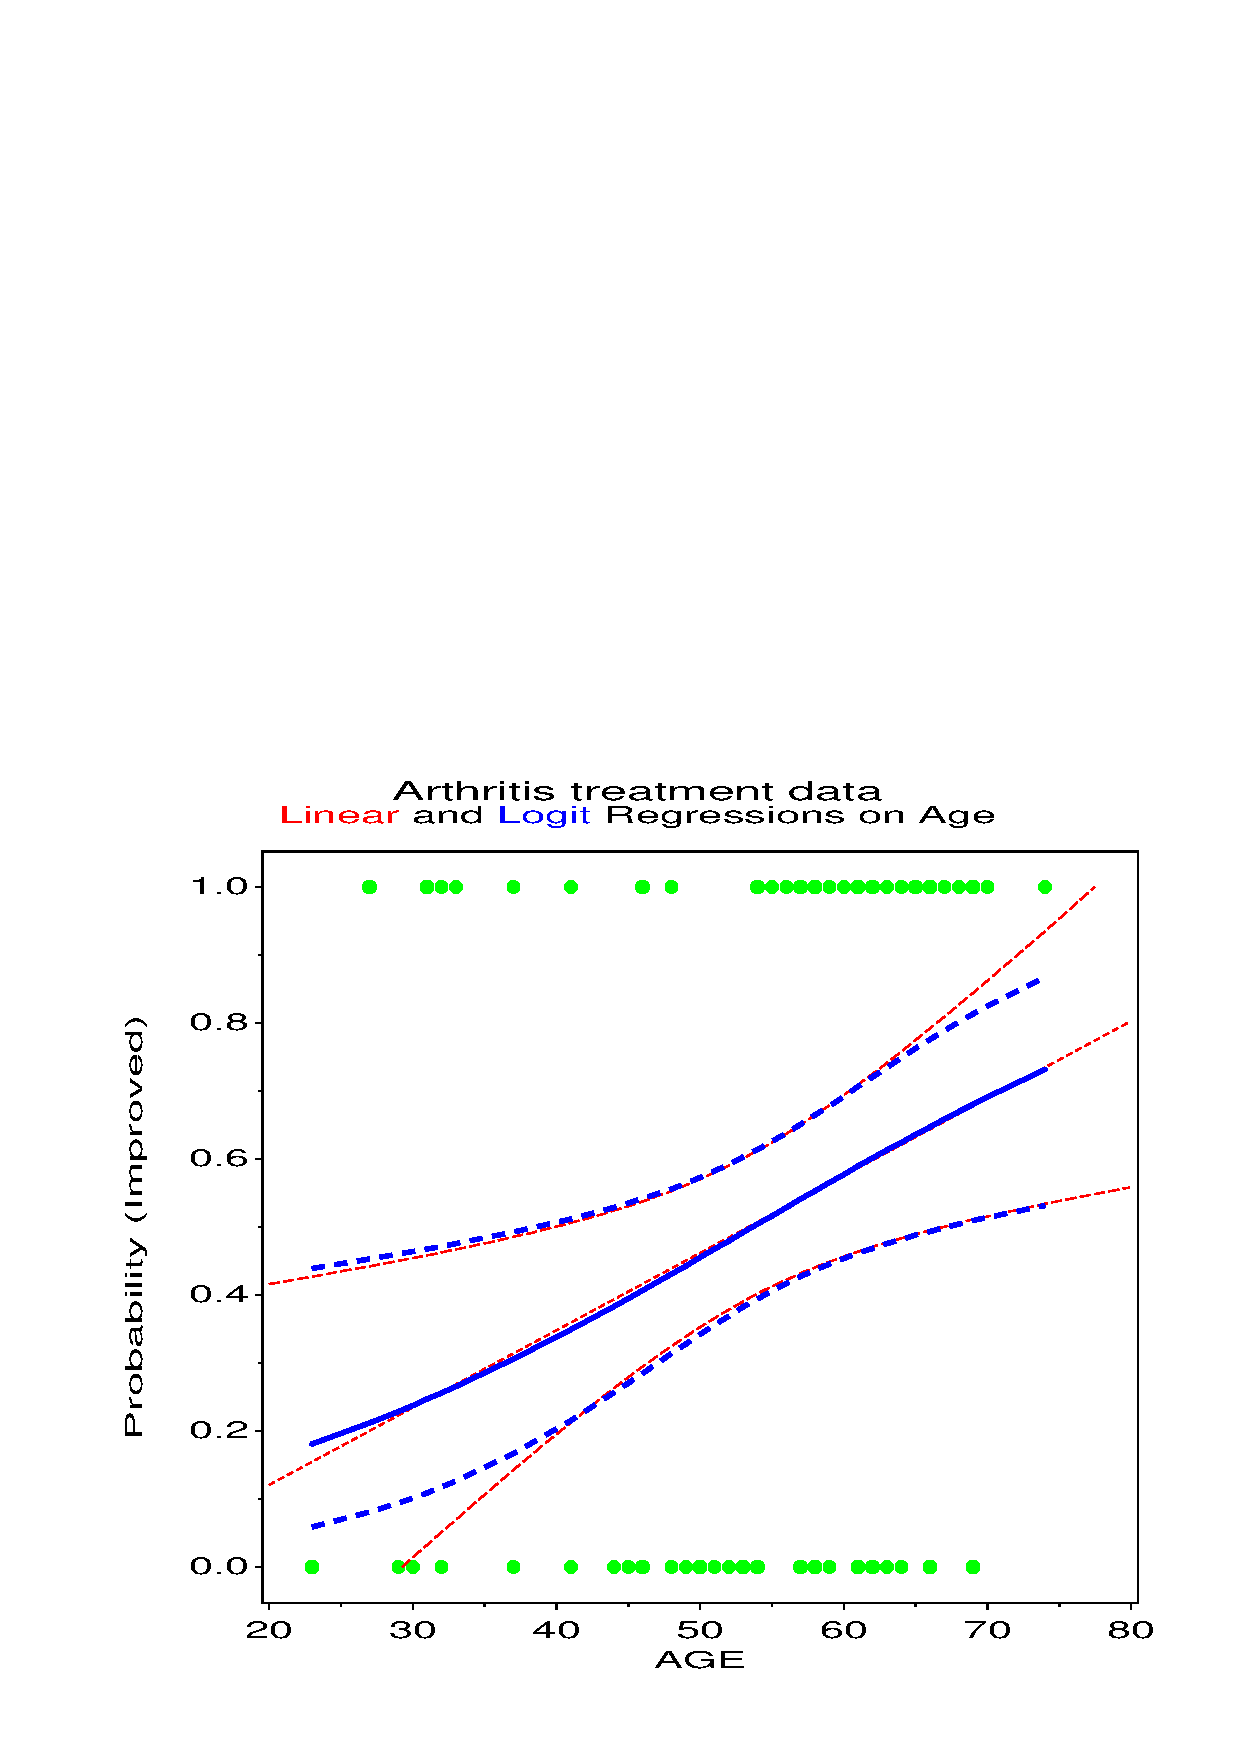
\includegraphics[height=0.7\textheight]{fig/logist1c1}
\end{center}

\end{frame}

\begin{frame}
  \frametitle{Logistic regression models: Binary response}
  \begin{itemize}[<+->]
	\item For a binary response, $Y \in (0,1)$, 
	let 
	\vec{x} be a vector of $p$ regressors, and  
	$\pi_i$ be the probability, $\Pr (Y=1 \given \vec{x})$. 
	\item The logistic regression
	model is a linear model for the \emph{log odds}, or \emph{logit}
	that $Y=1$, given the values in \vec{x},
\begin{eqnarray*}
  \logit ( \pi_{i}) \equiv \log \left( \frac{\pi_i}{1 - \pi_i}  \right)
   &=& \alpha + \vec{x}_{i}\trans \,  \vec{\beta} \\ % \label{eq:logisr}
   &=& \alpha + \beta_1 x_{i1} + \beta_2 x_{i2} + \cdots + \beta_p x_{ip}
   \nonumber
\end{eqnarray*}
	\item An equivalent (non-linear) form of the model may be specified for
	the probability,  $\pi_i$, itself,
\begin{equation*}
    \pi_i = {\{ 1 + \exp ( -[\alpha + \vec{x}_{i}\trans \,  \vec{\beta} ] ) \}}^{-1}
\end{equation*}

	\item The logistic model is a \emph{linear model} for the log odds, but also a
	\emph{multiplicative} model for the odds of ``success,''
\begin{equation*}
\frac{\pi_i}{1 - \pi_i} = \exp( \alpha + \vec{x}_{i}\trans \,  \vec{\beta} )
   = \exp(\alpha) \exp ( \vec{x}_{i}\trans \,  \vec{\beta} )
\end{equation*}
so, increasing $x_{ij}$ by 1 increases $\logit ( \pi_{i})$ by $\beta_j$,
and multiplies the odds by $e^{\beta_j}$.
%	\item Other ``link functions,'' transforming the probability, $\pi_i$,
%	to the ``linear predictor'' are possible (probit, complementary log-log)   
  \end{itemize}
\end{frame}


\renewcommand{\FileName}{logistic2}

\subsection{Fitting logistic models}
\begin{frame}[fragile]
  \frametitle{Logistic regression models: Binary response}
  \begin{block}{\large\bfseries Fitting} \PROC{LOGISTIC} (or \macro{ROBUST}--- M-estimation)
     \begin{itemize*}
	    \item Data:
    	\begin{itemize*}
		   \item Frequency form (from \PROC{FREQ})--- when all predictors are discrete
		   \item Case form--- when any predictors are quantitative
		  \end{itemize*}
	  \item Models:  
    	\begin{itemize*}
		\item \stmt{CLASS} (V7+)--- no need for dummy variables
    	   \begin{itemize*}
		   \item discrete predictors
		   \item can specify \emph{order} and \emph{parameterization} (effect, polynomial, reference
		   cell)
		   \end{itemize*}
		\item \stmt{MODEL}--- allows \texttt{GLM} syntax, e.g., 

\begin{listing}[frame=single]
proc logistic;
  class Sex Treat;
  model Better = Sex | Treat | Age @2;
\end{listing}

		\item $\Rightarrow$ \texttt{Better = Sex Treat Age Sex*Treat Sex*Age Treat*Age}
		\end{itemize*}
	  \end{itemize*}
  \end{block}
\end{frame}

\subsection{Visualizing logistic models}
\begin{frame}
  \frametitle{Logistic regression models: Binary response}
  \begin{block}{\large\bfseries Visualization}
    \begin{itemize*}
	  \item Goal: \emph{see} and \emph{understand} the data and fitted model
	  \item \macro{LOGODDS}: Plot observed responses, fitted and smoothed probabilities
	  \item Model plots:
    	\begin{itemize*}
		    \item \stmt{OUTPUT} $\rightarrow$ 
    	   \begin{itemize*}
			    \item fitted $\hat{\pi}_i$, lower/upper $(1-\alpha)$ CI, and/or 
			    \item fitted logit, $(\alpha + \vec{x}_{i}\trans \,  \hat{\vec{\beta}}) \pm
			      z_{1-\alpha/2} se(\logit)$
    	   \end{itemize*}
			
		\item Plot with standard procedures (\PROC{GCHART}, \proc{GPLOT})
		\item Utility macros (\pname{BARS}, \pname{LABEL}, \pname{POINTS}, \pname{PSCALE}, etc.)
		for custom displays
		\end{itemize*}
	  \item Effect plots--- plot hierarchical subset of effects, averaging over
	  those not included.
	  \item \macro{INFLOGIS}: Influence plots for logistic regression models
	  \item \macro{ADDVAR}: Added variable plots for new predictors or transformations of old
	  \end{itemize*}
  \end{block}
\end{frame}


\begin{frame}[fragile]
  \frametitle{Example: Arthritis treatment data}
  \begin{itemize}
  	\item \alert{Predictors}: Sex, Treatment (treated, placebo), Age
	\item \alert{Response}: improvement (none, some, marked)
      \begin{itemize*}
	  \item Consider first as binary response: None vs. (Some or Marked)=`Better'
	  \end{itemize*}
	\item Data in case form:
  \end{itemize}
\begin{Input}[fontsize=\small,label=\fbox{\texttt{arthrit.sas}},baselinestretch=0.7]
data arthrit;
   length treat $7. sex $6. ;
   input id treat $ sex $ age improve @@ ;
   case = _n_;
   \sasemph{better  = (improve > 0);}  \sascomment{*-- Make binary response;}
datalines ;
57 Treated Male   27 1   9 Placebo Male   37 0
46 Treated Male   29 0  14 Placebo Male   44 0
77 Treated Male   30 0  73 Placebo Male   50 0
  ... (\emph{observations omitted})
56 Treated Female 69 1  42 Placebo Female 66 0
43 Treated Female 70 1  15 Placebo Female 66 1
                        71 Placebo Female 68 1
                         1 Placebo Female 74 2
;
\end{Input}
\end{frame}

\subsection{Empirical logit plots}
\begin{frame}[fragile]
  \frametitle{\macrot{LOGODDS}: Empirical logit plots}
  Problems with visualizing discrete outcomes:
  \begin{itemize}
	\item{\large\bfseries Linearity}: Is a linear relation realistic?
	\item{\large\bfseries Smoothing}: Discrete data often requires smoothing to see!
  \end{itemize}

The \macro{LOGODDS}:
   \begin{itemize*}
   \item Show the data: Plot (0/1) responses [stacked or jittered]
   \item Divide $X$ into groups (e.g., deciles), emprical logit,
   $\log \left(\frac{y_i + 1/2}{n_i - y_i + 1/2}\right)$,
   for each
   \item Linear logistic regression, plus smoothed curve (\macro{LOWESS})
   \end{itemize*}
\vspace{1ex}
\begin{Input}
%include catdata(arthrit);
%logodds(data=arthrit, 
    x=age, y=Better,  \sascomment{/* vars to plot               */}
    smooth=0.5,       \sascomment{/* LOWESS smoothing parameter */}
    plot=logit);      \sascomment{/* plot on logit scale        */}
\end{Input}
\end{frame}

\begin{frame}
\begin{center}
  \includegraphics[width=.9\dispwidth,clip]{fig/logoddt}
\end{center}
\end{frame}

\begin{frame}
\frametitle{Smoothing the binary observations}
Can also use direct smoothing:
\begin{center}
  \includegraphics[width=.6\dispwidth,clip,trim=0 15 0 25]{fig/arthritis-lowess}
\end{center}
\begin{itemize*}
 \item SAS: \PROC{LOESS}, \macro{lowess}; R: \func{lowess}
 \item There is a hint that the relation may be non-linear
 \item But data is thin at the extremes
\end{itemize*}

\end{frame}

%\endinput
\subsection{PROC LOGISTIC: Fitting and plotting}
\begin{frame}[fragile]
  \frametitle{\PROC{LOGISTIC}: Model fitting and plotting}
  \begin{itemize}
	\item Specify ordering of response levels (\texttt{order=} or \texttt{descending} options)
	\item Specify parameterizations for \texttt{CLASS} variables
	\item \stmt{OUTPUT} to get fitted logits and probabilities
  \end{itemize}
  \vspace{1ex}
\begin{Input}[label=\fbox{\texttt{glogist1c.sas} $\cdots$},baselinestretch=0.7]
\vspace{.2ex}
proc logistic data=arthrit \sasemph{descending};
   \sasemph{class sex (ref=last) treat (ref=first) / param=ref};
   model better = sex  treat  age;
   \sasemph{output} out=results 
          p=prob l=lower u=upper
          xbeta=logit stdxbeta=selogit / alpha=.33;
\end{Input}
The output includes:
\begin{Output}[gobble=5,fontsize=\small,baselinestretch=0.8]
                    Type III Analysis of Effects
 
                                     Wald
             Effect      DF    Chi-Square    Pr > ChiSq

             sex          1        6.2576        0.0124
             treat        1       10.7596        0.0010
             age          1        5.5655        0.0183
\end{Output}
\end{frame}

\begin{frame}[fragile]
\begin{Output}[gobble=1,fontsize=\footnotesize]
             Analysis of Maximum Likelihood Estimates
 
                                  Standard        Wald
 Parameter          DF  Estimate     Error  Chi-Square  Pr > ChiSq

 Intercept           1   -4.5033    1.3074     11.8649      0.0006
 sex       Female    1    \sasemph{1.4878}    0.5948      6.2576      0.0124
 treat     Treated   1    \sasemph{1.7598}    0.5365     10.7596      0.0010
 age                 1    \sasemph{0.0487}    0.0207      5.5655      0.0183

                        Odds Ratio Estimates
                                  
                                   Point          95% Wald
    Effect                      Estimate      Confidence Limits

    sex   Female vs Male           \sasemph{4.427}       1.380      14.204
    treat Treated vs Placebo       \sasemph{5.811}       2.031      16.632
    age                            \sasemph{1.050}       1.008       1.093
\end{Output}
Parameter estimates (reference cell coding):
\begin{itemize*}
  \item $\beta_1 = 1.49 \Rightarrow$ Females $e^{1.49}$=4.43 $\times$ more likely better than Males
  \item $\beta_2 = 1.76 \Rightarrow$ Treated $e^{1.76}$=5.81 $\times$ more likely better than Placebo
  \item $\beta_3 = 0.0487 \Rightarrow$ odds ratio=1.05 $\Rightarrow$ odds of improvement
  increase 5\% each year.  Over 10 years, odds of improvement
  $= e^{10 \times 0.0486}= 1.63$, a 63\% increase.  
\end{itemize*}
\end{frame}

\begin{frame}[fragile]
  \frametitle{\PROC{LOGISTIC}: Full-model plots}
 \alert{Full-model plots} display the fitted (predicted) values over \emph{all combinations}  ofpredictors:
  \begin{itemize}
	\item Plot fitted values from the \Dset\ specified on the \stmt{OUTPUT}
	\item Plot either predicted probabilities or logits
	\item Confidence intervals or standard errors allow showing error bars
  \end{itemize}
The first few observations from the \texttt{results} \Dset:
\begin{Output}[gobble=2,fontsize=\footnotesize]
   id sex   treat  age better   prob  lower  upper  logit selogit

   57 Male Treated  27    1    0.194  0.103  0.334 -1.427  0.758 
    9 Male Placebo  37    0    0.063  0.032  0.120 -2.700  0.725 
   46 Male Treated  29    0    0.209  0.115  0.350 -1.330  0.728 
   14 Male Placebo  44    0    0.086  0.047  0.152 -2.358  0.658 
   77 Male Treated  30    0    0.217  0.122  0.357 -1.281  0.713 
   73 Male Placebo  50    0    0.112  0.065  0.188 -2.066  0.622 
    ...
\end{Output}
  \begin{itemize*}
	\item \texttt{prob}-- predicted probabilities, with CI (\texttt{lower} ,\texttt{upper} )
	\item \texttt{logit}-- predicted logit, with standard error \texttt{selogit} 
  \end{itemize*}

\end{frame}

\begin{frame}[fragile]
  \frametitle{\PROC{LOGISTIC}: Full-model plots}
Basic plots:
  \begin{itemize*}
	\item Plot either logit or probability vs. one predictor (continuous or most levels)
	\item Separate curves for one factor (\texttt{= factor})
	\item Separate panels for all others (\stmt{BY})
  \end{itemize*}

\begin{Input}
proc gplot data=results;
   plot (logit prob) * age = \sasemph{treat};     \sascomment{/* separate curves */}
   \sasemph{by sex;}                              \sascomment{/* separate panels */}
   symbol1 v=circle i=join l=3 c=black; \sascomment{/* placebo */}
   symbol2 v=dot    i=join l=1 c=red;   \sascomment{/* treated */}
\end{Input}
  \begin{itemize*}
	\item \stmt{SYMBOL}--- define the point value (\texttt{v=}), interpolate option (\texttt{i=}), line style (\texttt{l=}), 
	color (\texttt{c=}), etc. 
  \end{itemize*}

\end{frame}

\begin{frame}
  \frametitle{\PROC{LOGISTIC}: Model plots}
Enhanced plots:

  \begin{itemize*}
	\item Plot on logit scale, with probability scale at right (\macro{PSCALE})
	\item Show 67\% error bars $\approx \pm 1$ se (\macro{BARS})
	\item Custom legend and panel labels (\macro{LABEL})
  \end{itemize*}

 \begin{center}
  \includegraphics[width=1\dispwidth,clip]{fig/glogist1c}
 \end{center}

\end{frame}

\begin{frame}[fragile]
  \frametitle{\PROC{LOGISTIC}: Full-model plots}
Enhanced plots:

\begin{Input}[fontsize=\footnotesize,label=\fbox{$\cdots$ \texttt{glogist1c.sas} $\cdots$},baselinestretch=0.7,firstnumber=9]
  \sascomment{*-- Error bars, on logit scale;}
%bars(data=results, var=logit, 
   class=age, cvar=treat, by=age,
   barlen=selogit, \sasemph{out=bars});

  \sascomment{*-- Custom legends and panel labels;}
%label(data=results, y=logit, x=age, xoff=1, cvar=treat,
   by=sex, subset=last.treat, \sasemph{out=label1}, pos=6, text=treat);
%label(data=results, y=2.5, x=20, size=2,
   by=sex, subset=first.sex, \sasemph{out=label2}, pos=6, text=sex);

  \sascomment{*-- Probability scales at right;}		
%pscale(\sasemph{out=pscale}, 
   byvar=sex, byval=%str('Female','Male'));

  \sascomment{*-- Join ANNOTATE datasets;}		
data \sasemph{bars};
   set \sasemph{label1 label2 bars pscale};
proc sort;
   by sex;
\end{Input}
\end{frame}

\begin{frame}[fragile]

\begin{Input}[fontsize=\footnotesize,label=\fbox{$\cdots$ \texttt{glogist1c.sas}},baselinestretch=0.7,firstnumber=30]
title ' '
   h=1.8 a=-90 'Probability Improved'    \sascomment{/* right axis label   */}
   h=2.5 a=-90 ' ';                      \sascomment{/* extra space        */}
goptions hby=0;                          \sascomment{/* suppress BY values */}
proc gplot data=results;
   plot \sasemph{logit * age = treat} / 
         vaxis=axis1 haxis=axis2 hm=1 vm=1
         nolegend \sasemph{anno=bars} frame;
   \sasemph{by sex;}
   axis1 label=(a=90 'Log Odds Improved')
         order=(-3 to 3);
   axis2 order=(20 to 80 by 10) offset=(2,6);
   symbol1 v=+ i=join l=3 c=black;
   symbol2 v=- i=join l=1 c=red;
   label age='Age';
run;
\end{Input}
 \begin{center}
  \includegraphics[width=.6\dispwidth,clip]{fig/glogist1c}
 \end{center}
\end{frame}

\begin{frame}[fragile]
  \frametitle{Models with interactions}
  \begin{itemize}
	\item{\large\bfseries Plotting fitted values}
      \begin{itemize*}
	  \item Only need to change the \stmt{MODEL}
	  \item Output \Dset\ automatically incorporates all model terms
	  \item Plotting steps remain \emph{exactly} the same
    \end{itemize*}
  \end{itemize}
\begin{Input}[baselinestretch=0.8,fontsize=\footnotesize]
proc logistic data=arthrit descending;
   class sex (ref=last) treat (ref=first) / param=ref;
   \sasemph{model  better = treat sex  | age @2;};
   output out=results p=prob l=lower u=upper
          xbeta=logit stdxbeta=selogit / alpha=.33;
\end{Input}

 \begin{center}
  \includegraphics[width=.7\dispwidth,clip]{fig/glogist1e}
 \end{center}
\end{frame}

\endinput
% slide template
\begin{frame}
  \frametitle{}
  \begin{itemize}
	\item{\large\bfseries }
      \begin{itemize*}
	  \item 
    	\begin{itemize*}
		\item 
		\item 
		\end{itemize*}
	  \item 
	  \end{itemize*}
	\item{\large\bfseries }
	\item{\large\bfseries }
  \end{itemize}
\end{frame}


\section{Effect plots}
\renewcommand{\FileName}{effplot}
\subsection{General ideas}
\begin{frame}
 \frametitle{Effect plots: basic ideas}
Show a given effect (and low-order relatives) coltrolling for other model effects.
\begin{center}
 \includegraphics[width=.80\textwidth]{fig/effect-demo}
\end{center}
\end{frame}
 
\begin{frame}
  \frametitle{Effect plots for generalized linear models}
  \begin{itemize}
    \item For simple models, full model plots show the complete relation between response
	and all predictors.
	\item \citet{Fox:87}--- For complex models, often wish to plot a specific main effect or
	interaction (including lower-order relatives)--- controlling for other effects
      \begin{itemize*}
	  \item Fit full model to data with linear predictor (e.g., logit) $\vec{\eta} = \mat{X} \vec{\beta}$ and link function
	  $g(\vec{\mu}) = \vec{\eta} $ $\rightarrow$ estimate $\vec{b}$ of $\vec{\beta}$ and covariance matrix
	  $\widehat{V(\vec{b})}$ of  $\vec{b}$.
	  \item Vary each predictor in the term over its' range
	  \item Fix other predictors at ``typical'' values (mean, median, proportion in the data)
	  \item $\rightarrow$ ``effect model matrix,'' $\mat{X}^*$
	  \item Calculate fitted effect values, $\hat{\vec{\eta}}^* = \mat{X}^* \vec{b}$.
	  \item Standard errors are square roots of $\diag{\mat{X}^* \widehat{V(\vec{b})} {\mat{X}^*}\trans }$
	  \item Plot $\hat{\vec{\eta}}^*$, or values transformed back to scale of response, $g^{-1} (\hat{\vec{\eta}}^*)$.
	  \end{itemize*}
	\item \emph{Note}: This provides a general means to visualize interactions in \emph{all} linear and generalized
	linear models.
  \end{itemize}
  
\end{frame}

\subsection{Effect plot in SAS}
\begin{frame}
  \frametitle{Effect plots in SAS}
  \begin{itemize}
%    \item SAS 9.2 ODS Graphics
%  	\begin{itemize*}
% 		\item Several procedures now do effects-like plots: LOGISTIC, GLM, GLIMMIX
%         \item Easy, but limited in what you can plot
% 	\end{itemize*}
  \item General method
	\begin{itemize*}
		\item Create a grid of values for predictors in the effect (\macro{EXPGRID})
		\item Fix other predictors at ``typical'' values (mean, median, proportion in the data)
		\item Concatenate grid with data
		\item Fit model $\rightarrow$ output data set $\rightarrow$ fitted values in the grid
		\item Standard errors automatically calculated
		\item Plot fitted values in the grid
	\end{itemize*}
  \item \macro{EFFPLOT}
	\begin{itemize*}
		\item Works with \PROC{REG}, \PROC{GLM}, \PROC{LOGISTIC}, \PROC{GENMOD}
		\item Uses \macro{MEANPLOT} to do the plotting -- some limitations
	\end{itemize*}

  \end{itemize}


\end{frame}

\begin{frame}
  \frametitle{Effect plots: Example}
  \begin{itemize}
	\item \citet{CowlesDavis:87}--- Volunteering for a psychology experiment
      \begin{itemize*}
	  \item Predictors: Sex, Neuroticism, Extraversion
	  \item $\rightarrow$ strong interaction, Neuroticism $\times$ Extraversion
	  \end{itemize*}
  \end{itemize}

 \begin{center}
  \includegraphics[width=.7\dispwidth,clip,trim=0 0 0 25]{fig/cowles3}
 \end{center}

\end{frame}

\begin{frame}[fragile]
  \frametitle{Effect plots: Example}
\begin{Input}[fontsize=\footnotesize,label=\fbox{\texttt{cowles3.sas}},baselinestretch=0.8]
%include catdata(cowles);
%expgrid(Sex=0.5,         \sascomment{/* Fix Sex at mid value */}
   Extraver=0 to 24 by 3, \sascomment{/* range of predictors  */} 
   Neurot=0 to 24 by 6,   \sascomment{/*    "          "      */}
   \sasemph{_in_=1});               \sascomment{/* grid select value  */}

\sascomment{*-- catenate grid values with data;}
data cowles;
   set cowles _grid_;

\sascomment{*-- fit model, output fitted values;}
proc logistic data=cowles outest=parm covout;
   model Volunter = Sex Extraver | Neurot  / covb;
   output out=predicted xbeta=logit stdxbeta=selogit 
      p=prob u=upper l=lower / alpha=.33;

\sascomment{*-- select grid, replace labels;}
data effect;
   set predicted (\sasemph{where =(_in_=1)});
   label logit='log odds of Volunteering'
      prob = 'Probability of Volunteering';
\end{Input}

\end{frame}

\begin{frame}[fragile]
  \frametitle{Effect plots: Example}
\begin{Input}[fontsize=\footnotesize,label=\fbox{$\cdots$ \texttt{cowles3.sas}},baselinestretch=0.75,firstnumber=23]
\sascomment{*-- Custom legend;}
%label(data=effect, 
   x=Extraver, y=prob, 
   subset=Extraver=24,       \sascomment{/* at last.Extraver */}
   text=put(Neurot,3.),      \sascomment{/* label text       */}
   pos=6, xoff=.2, \sasemph{out=labels});

\sascomment{*-- Plot step;}
proc gplot data=effect;
   plot \sasemph{prob * Extraver = Neurot} / 
      vaxis=axis1 haxis=axis2 vm=1
      \sasemph{anno=labels nolegend};
   symbol v=dot i=spline r=5;
   axis1 label=(a=90 r=0) order=(0 to .9 by .1);
   axis2 order=(0 to 30 by 6) offset=(3,1);
run; quit;
\end{Input}
 \begin{center}
  \includegraphics[width=.35\dispwidth,clip,trim=0 0 0 25]{fig/cowles3}
 \end{center}

\end{frame}

\subsection{The effects package in R}
% slide template
\renewcommand{\FileName}{Cowles}
\begin{frame}[fragile]
  \frametitle{Effect plots with the \texttt{effects} package in R}
\begin{Rin}
> library(effects)  ## load the effects package 
> data(Cowles)
> mod.cowles <- glm(volunteer ~ sex + neuroticism*extraversion, 
+     data=Cowles, family=binomial)
> summary(mod.cowles)
\end{Rin}
\begin{Rout}[fontsize=\footnotesize,baselinestretch=0.9]
Coefficients:
                          Estimate Std. Error z value Pr(>|z|)    
(Intercept)              -2.358207   0.501320  -4.704 2.55e-06 ***
sexmale                  -0.247152   0.111631  -2.214  0.02683 *  
neuroticism               0.110777   0.037648   2.942  0.00326 ** 
extraversion              0.166816   0.037719   4.423 9.75e-06 ***
neuroticism:extraversion -0.008552   0.002934  -2.915  0.00355 ** 
---
Signif. codes:  0 '***' 0.001 '**' 0.01 '*' 0.05 '.' 0.1 ' ' 1 

(Dispersion parameter for binomial family taken to be 1)

    Null deviance: 1933.5  on 1420  degrees of freedom
Residual deviance: 1897.4  on 1416  degrees of freedom
AIC: 1907.4
\end{Rout}
\end{frame}

 
\begin{frame}[fragile]
  \frametitle{Effect plots with the \texttt{effects} package in R}
Calculate effects for all model terms, plot neuro:extra:
\begin{Rin}[fontsize=\footnotesize]
> eff.cowles <- allEffects(mod.cowles, 
+      xlevels=list(neuroticism=0:24, 
+                   extraversion=seq(0, 24, 8)))
> 
> plot(eff.cowles, 'neuroticism:extraversion', ylab="Prob(Volunteer)",
+     ticks=list(at=c(.1,.25,.5,.75,.9)), layout=c(4,1), aspect=1)
\end{Rin}
 \begin{center}
 \includegraphics[width=.95\textwidth,clip]{R/Cowles1}
 \end{center}

\end{frame}

\begin{comment}
> 
> plot(eff.cowles, 'neuroticism:extraversion', multiline=TRUE, 
+     ylab="Prob(Volunteer)")
\end{comment}

\section{Influence measures and diagnostic plots}
\renewcommand{\FileName}{loginfl}
\begin{frame}
  \frametitle{Influence measures and diagnostic plots}
  \begin{itemize}
	\item{\large\bfseries Leverage}: Potential impact of an individual case $\sim$ distance
	from the centroid in space of predictors
	\item{\large\bfseries Residuals}: Which observations are poorly fitted? 
	\item{\large\bfseries Influence}: Actual impact of an individual case $\sim$ leverage $\times$ residual
      \begin{itemize*}
	  \item \boldital{C}, \boldital{CBAR} -- analogs of Cook's D in OLS $\sim$ standardized change in
	  regression coefficients when $i$-th case is deleted.
		\item \boldital{DIFCHISQ}, \boldital{DIFDEV} -- $\Delta \chi^2$ when $i$-th case is deleted.
	  \end{itemize*}
  \end{itemize}
 \begin{center}
  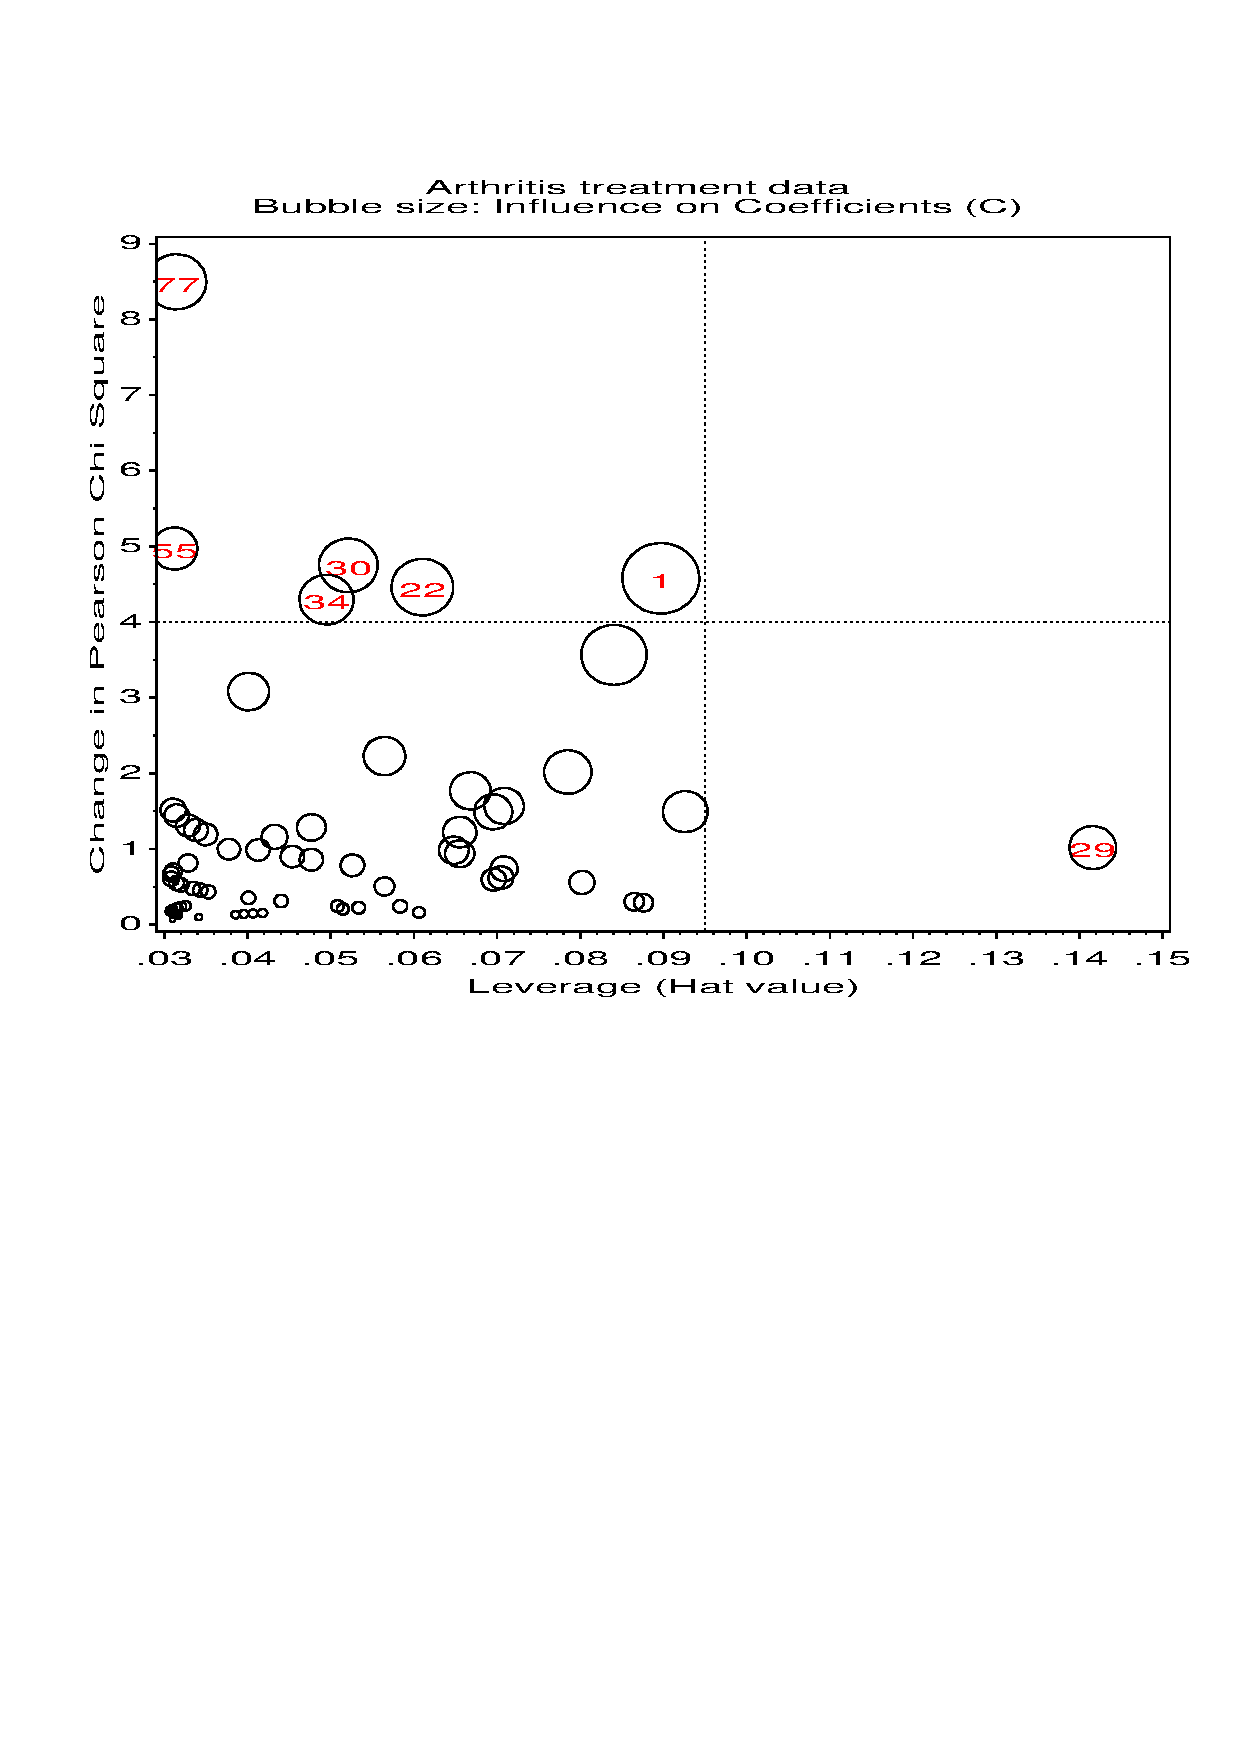
\includegraphics[width=.4\dispwidth,clip]{fig/logist1b2}
 \end{center}
\end{frame}

\begin{frame}[fragile,allowframebreaks]
  \frametitle{Influence measures and diagnostic plots}
\PROC{LOGISTIC}: printed output with the \texttt{influence} and \texttt{iplots} options
\begin{Input}
proc logistic data=arthrit ;
   model better = sex treat age / \sasemph{influence iplots};
\end{Input}

\begin{Output}[fontsize=\footnotesize,baselinestretch=0.6]
                     The LOGISTIC Procedure
                     Regression Diagnostics
          Deviance Residual               Hat Matrix Diagonal

Case             (1 unit = 0.26)               (1 unit = 0.01)
Number  Value   -8  -4  0 2 4 6 8     Value   0 2 4 6 8  12  16

   1    1.812  | *      |        |    0.089  |          *      |
   2    0.360  |        |*       |    0.031  |    *            |
   3    0.685  |        |  *     |    0.087  |          *      |
   4    0.425  |        | *      |    0.034  |    *            |
   5    0.700  |        |  *     |    0.086  |          *      |
   6    0.488  |        | *      |    0.038  |    *            |
   7    1.703  |  *     |        |    0.084  |         *       |
   8    0.499  |        | *      |    0.039  |    *            |
   9    1.396  |   *    |        |    0.066  |        *        |
  10    0.511  |        | *      |    0.040  |     *           |
  11    1.142  |    *   |        |    0.064  |       *         |
  12    0.523  |        | *      |    0.041  |     *           |
  13    1.234  |        |    *   |    0.065  |       *         |
  14    0.599  |        | *      |    0.051  |      *          |
  15    1.121  |    *   |        |    0.065  |       *         |
  16    0.599  |        | *      |    0.051  |      *          |
  17    1.319  |        |    *   |    0.069  |        *        |
  18    0.640  |        | *      |    0.058  |       *         |
  19    1.319  |        |    *   |    0.069  |        *        |
  20    0.640  |        | *      |    0.058  |       *         |
  21    1.340  |        |    *   |    0.070  |        *        |
  22    1.814  | *      |        |    0.061  |       *         |
  23    1.022  |    *   |        |    0.070  |        *        |
  24    0.529  |        | *      |    0.060  |       *         |
  25    1.449  |        |    *   |    0.078  |         *       |
  26    0.619  |        | *      |    0.053  |      *          |
  27    0.909  |     *  |        |    0.080  |         *       |
  ...
\end{Output}
Problems:
\begin{itemize*}
\item Way too much output
\item Doesn't highlight unusual cases well
\item Index plots don't consider combinations of measures
\end{itemize*}

\end{frame}

\subsection{INFLOGIS macro}
\begin{frame}
  \frametitle{\macrot{INFLOGIS}}
  \begin{itemize*}
	\item Specialized version of \macro{INFLGLIM} for logistic regression
	\item Plots a measure of change in $\chi^2$ (DIFCHISQ or DIFDEV) vs.\
	predicted probability or leverage.
	\item Bubble symbols show actual influence (C or CBAR)
	\item Shows standard cutoffs for ``large'' values
	\item Labels outlying cases
  \end{itemize*}
 \begin{center}
  \includegraphics[width=.95\dispwidth,clip]{fig/logist1b3}
 \end{center}

\end{frame}

\begin{frame}[fragile]
  \frametitle{\macrot{INFLOGIS}: Example}
\begin{Input}
%include data(arthrit);
%inflogis(data=arthrit,
   class=sex treat,      \sascomment{/* CLASS variables */}
   y=better,             \sascomment{/* response        */}
   x=sex treat age,      \sascomment{/* predictors      */}
   id=case,              \sascomment{/* case ID         */}
   gy=DIFCHISQ,          \sascomment{/* graph ordinate  */}
   gx=PRED HAT);         \sascomment{/* graph abscissas */}
\end{Input}
Printed output lists cases with ``large'' leverage, residual or influence:

\begin{Output}[gobble=4,fontsize=\footnotesize]
    case better  sex    treat  age pred  hat difchisq difdev    c

      1     1   Male   Treated  27 .806  .09   4.578   3.695  0.451
     22     1   Male   Placebo  63 .807  .06   4.460   3.565  0.290
     30     1   Female Placebo  31 .818  .05   4.749   3.657  0.261
     34     1   Female Placebo  33 .803  .05   4.296   3.464  0.224
     55     0   Female Treated  58 .172  .03   4.970   3.676  0.160
     77     0   Female Treated  69 .108  .03   8.498   4.712  0.276
\end{Output}
 
\end{frame}

\begin{frame}
  \frametitle{\macrot{INFLOGIS}: Example}
 \begin{center}
  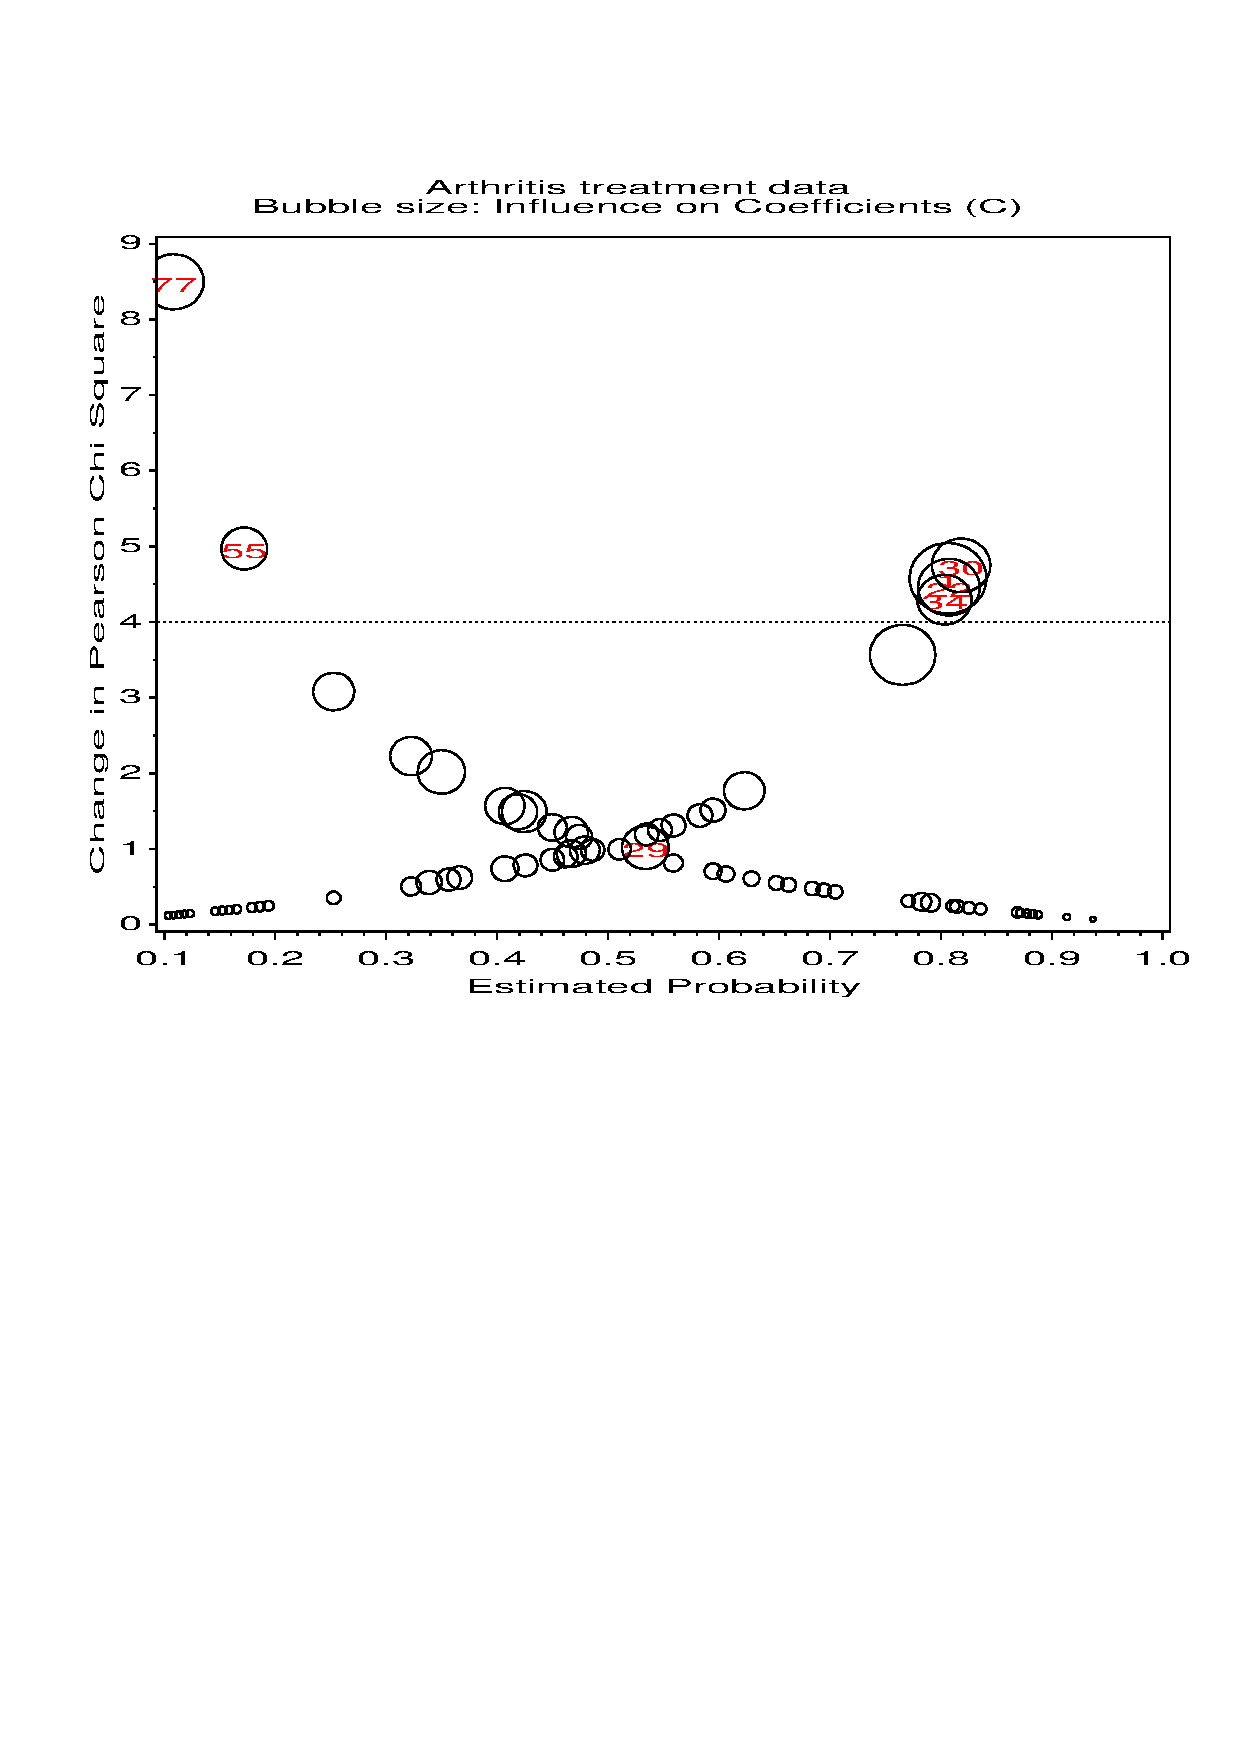
\includegraphics[width=.8\dispwidth,clip]{fig/logist1b1}
 \end{center}

\end{frame}

\begin{frame}
  \frametitle{\macrot{INFLOGIS}: Example}
 \begin{center}
  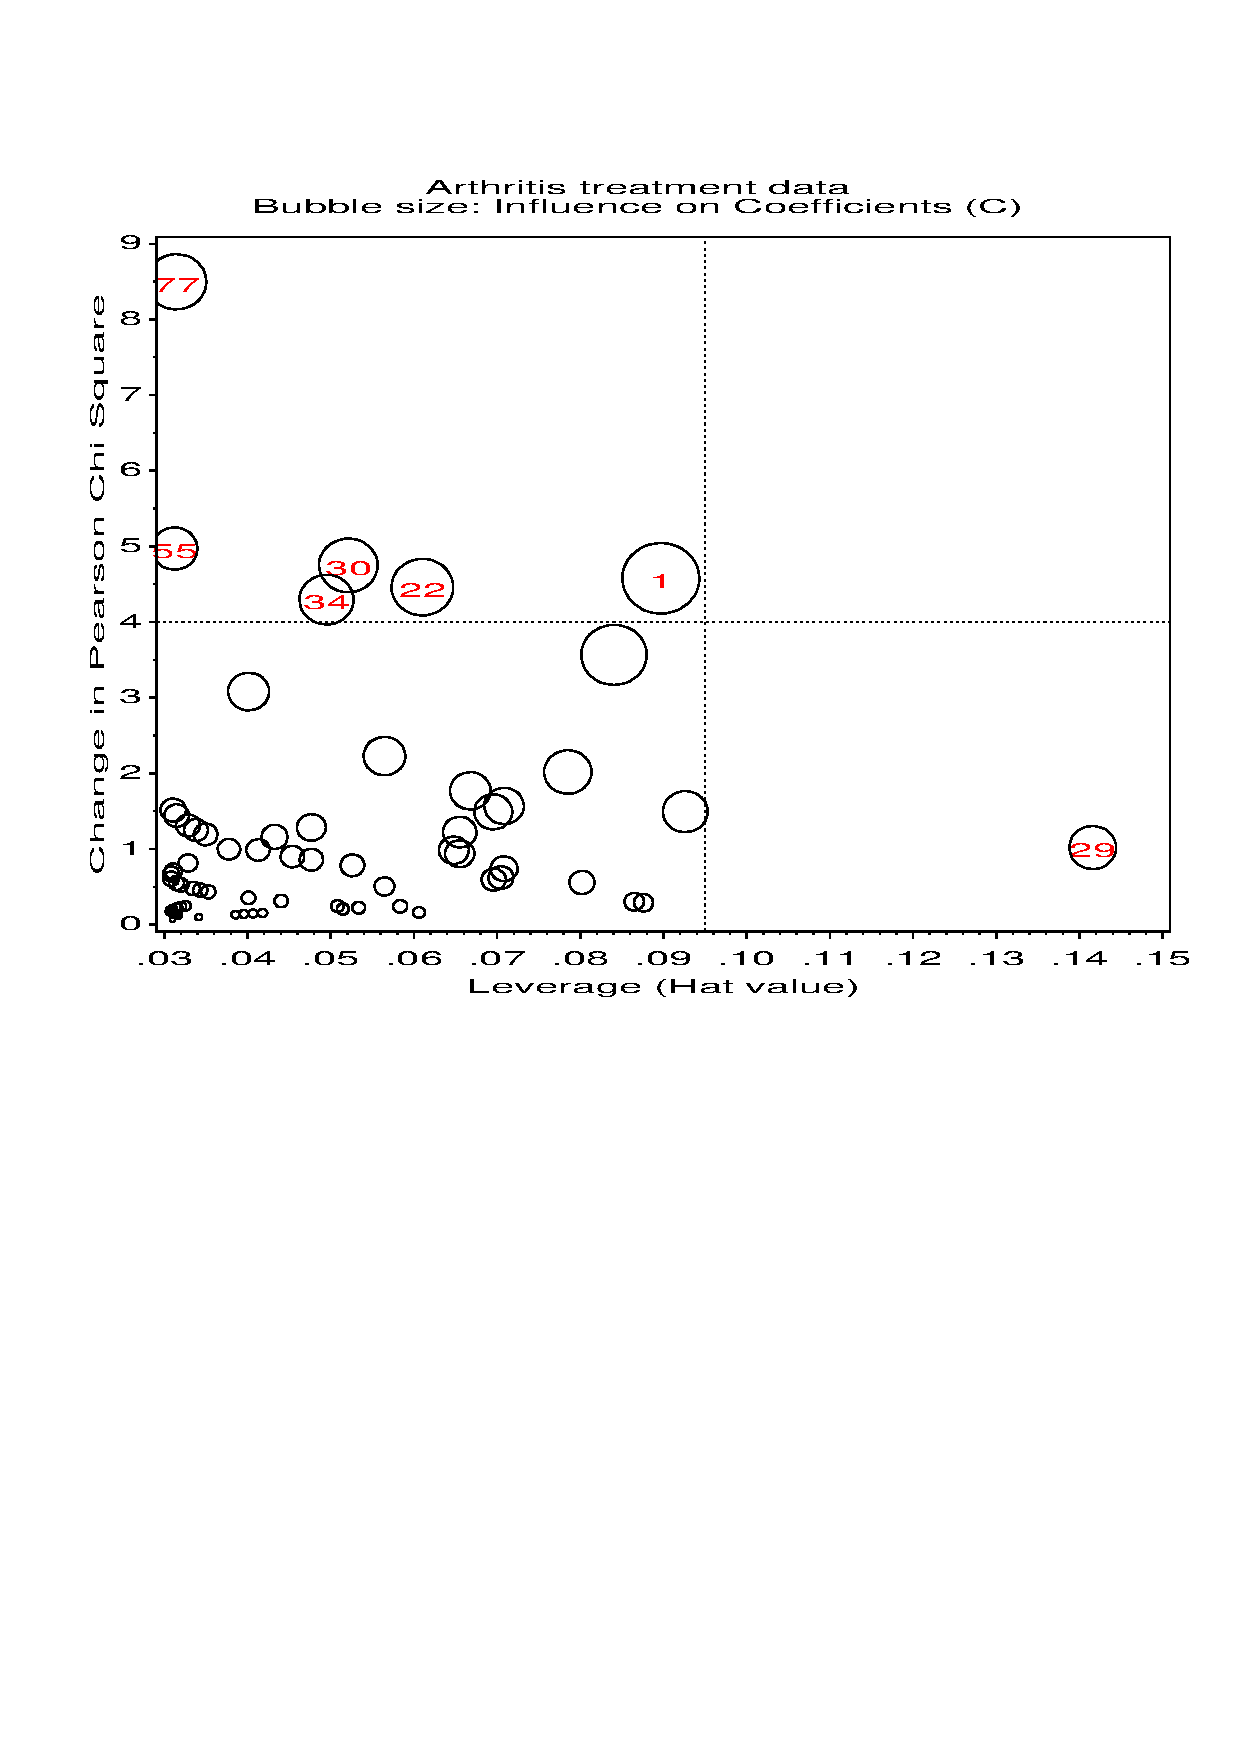
\includegraphics[width=.8\dispwidth,clip]{fig/logist1b2}
 \end{center}

\end{frame}
\subsection{Diagnostic plots in R}
\begin{frame}[fragile]
  \frametitle{Diagnostic plots in R}
In R, plotting a \texttt{glm} object gives the ``regression quartet''
\begin{Rin}[baselinestretch=0.8]
arth.mod1 <- glm(Better ~ Age+Sex+Treatment,data=Arthritis,
             family='binomial')
plot(arth.mod1) 
\end{Rin}

 \begin{center}
  \includegraphics[width=\dispwidth,clip,trim=0 0 0 10]{fig/arthritis-diag1a}
 \end{center}
\end{frame}

\begin{frame}[fragile]
  \frametitle{Diagnostic plots in R}
\begin{Rin}[baselinestretch=0.9]
library(car)
influencePlot(arth.mod1) 
\end{Rin}
 \begin{center}
  \includegraphics[width=.6\dispwidth,clip,trim=0 10 0 10]{fig/arthritis-diag2}
 \end{center}
\end{frame}


\part{Polytomous response}
\begin{frame}
  \frametitle{Part 5: Polytomous response models}
 \begin{minipage}[c]{.33\textwidth}
  \includegraphics[width=1\linewidth]{fig/catberk6}
  \end{minipage}%
 \hfill
 \begin{minipage}[c]{.33\textwidth}
  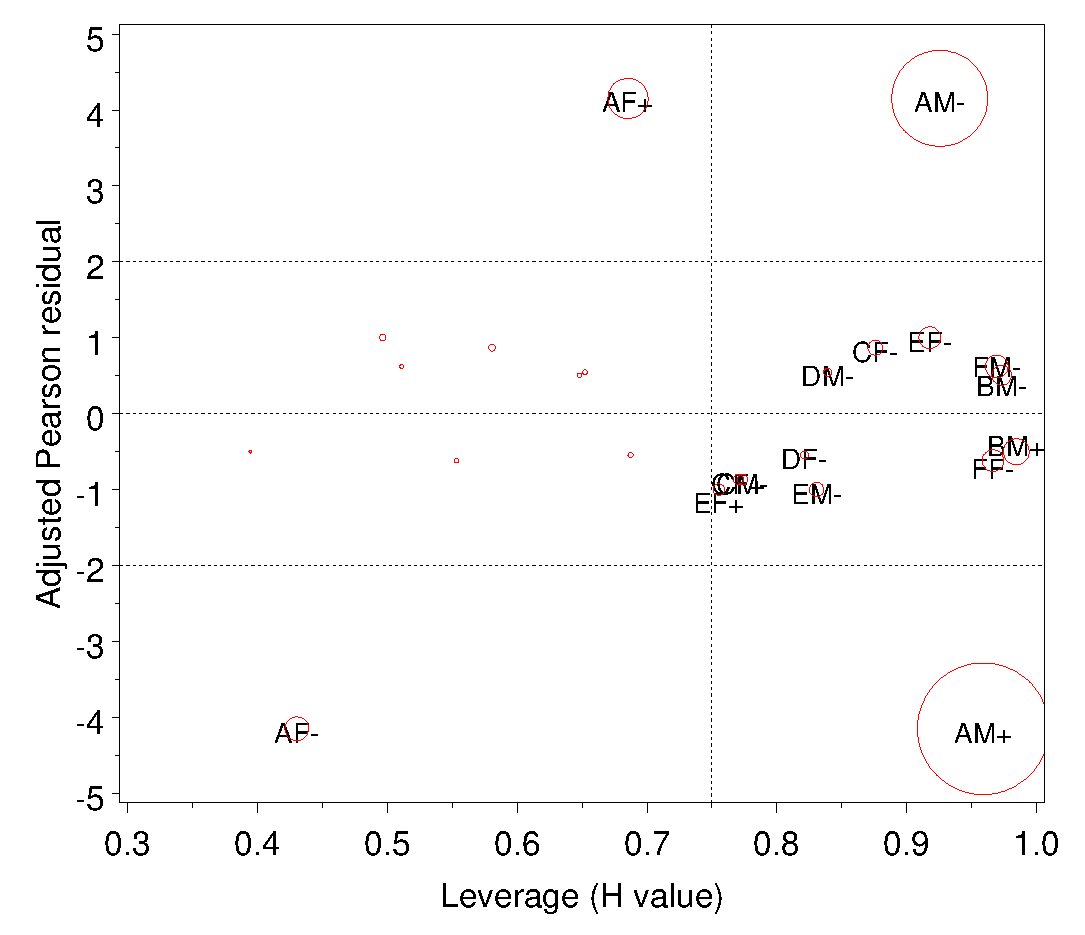
\includegraphics[width=1\linewidth,clip]{fig/genberk11}
 \end{minipage}
 \hfill
 \begin{minipage}[c]{.33\textwidth}
  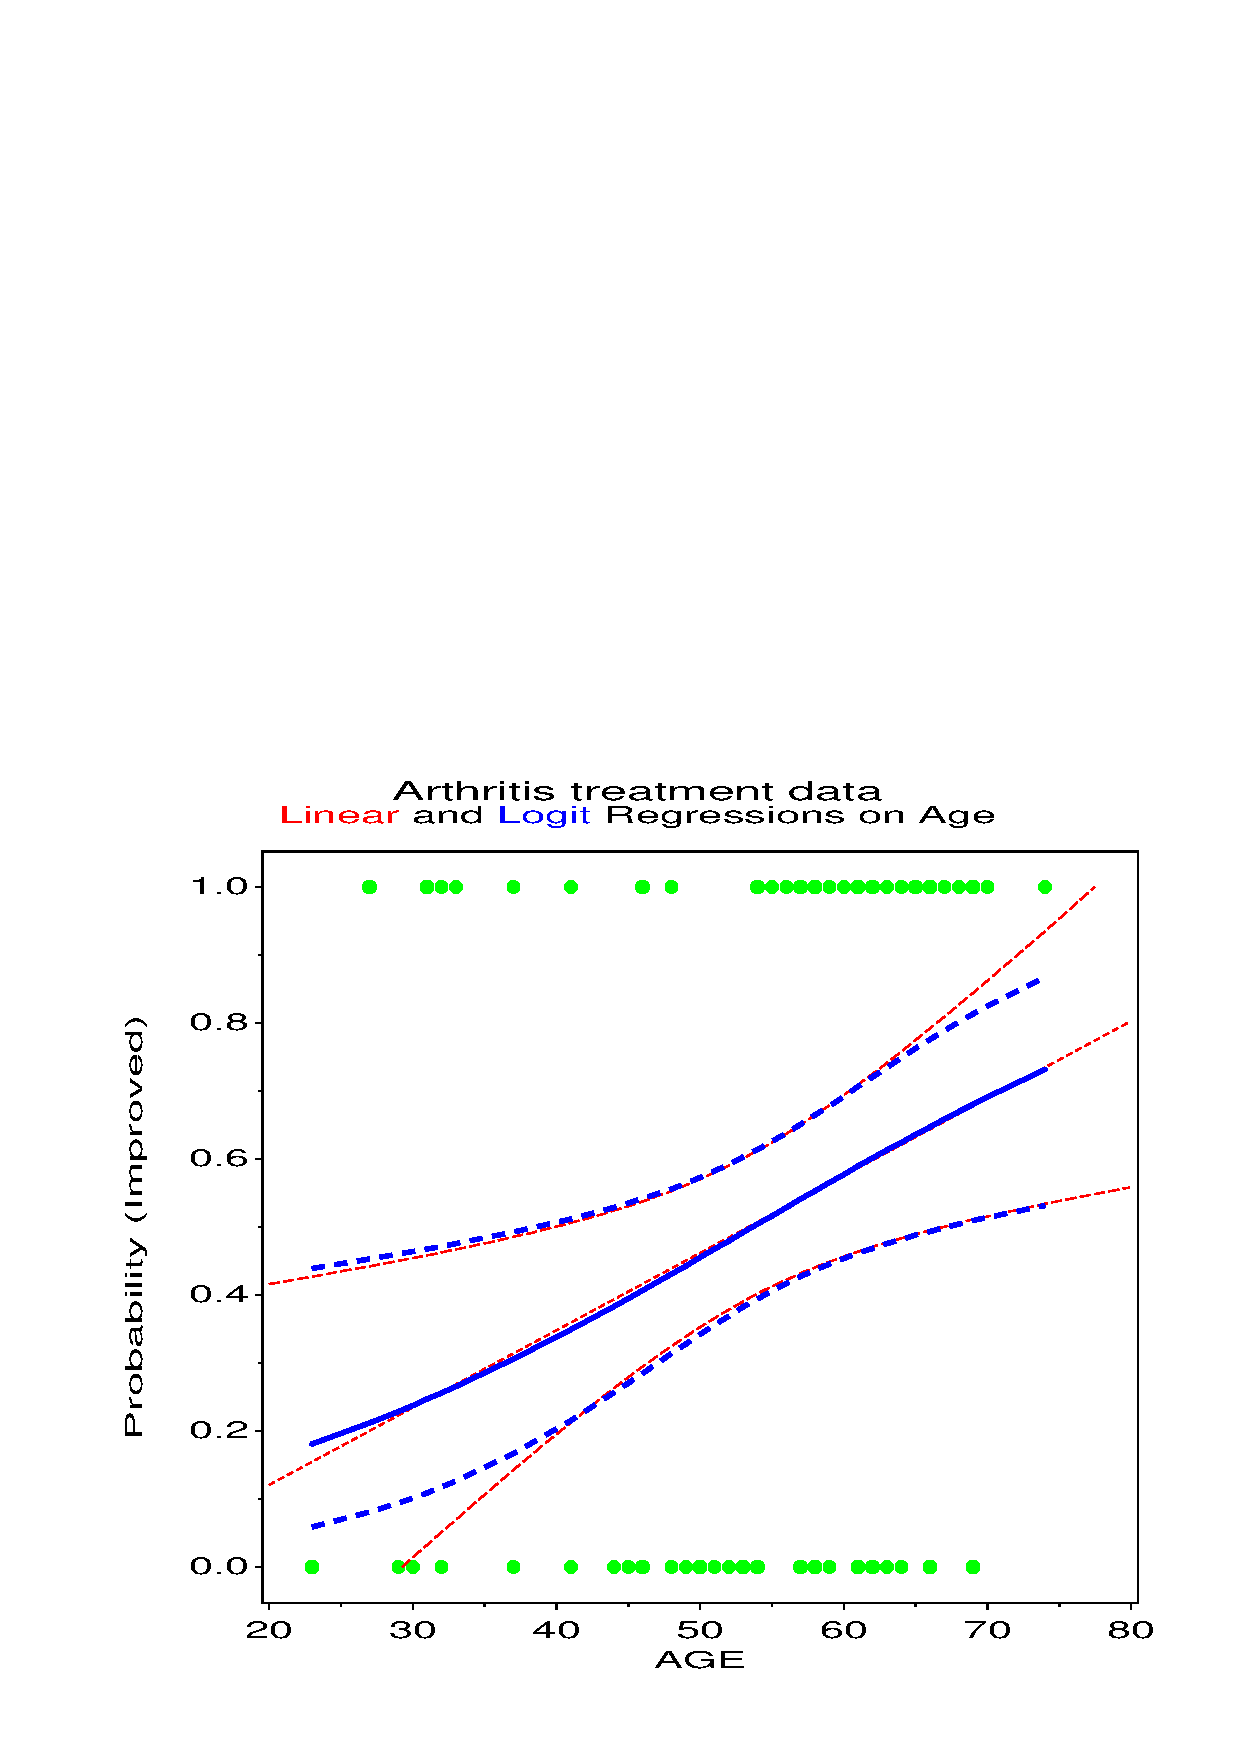
\includegraphics[width=1\linewidth,clip]{fig/logist1c1}
 \end{minipage}

Topics:
  \begin{itemize}
    \item 
	  \begin{itemize*} 
	    \item 
		\item 
	  \end{itemize*} 
	\item 
	  \begin{itemize*} 
	    \item 
		\item 
		\item 
	  \end{itemize*} 
  \end{itemize}
\end{frame}

\section{Polytomous response models}
\subsection{Overview}
\renewcommand{\FileName}{polytomous}
% slide template

\begin{frame}
  \frametitle{Polytomous responses: Overview}

\begin{center}
 \includegraphics[height=.8\dispheight]{fig/polytomous2}
\end{center}
 
\end{frame}

\begin{frame}
  \frametitle{Polytomous responses: Overview}
  \begin{itemize}
    \item<1-> $m$ categories $\rightarrow (m-1)$ comparisons (logits)
	\item<2->{\bfseries Response categories \emph{ordered}}, e.g., None, Some, Marked improvement
      \begin{itemize*}
	  \item Proportional odds model
    	\begin{itemize*}
		\item Uses adjacent-category logits
\begin{tabular}{l}
\fbox{None}  \fbox{ Some or Marked} \\
\fbox{None or Some}  \fbox{ Marked}
\end{tabular}

		\item Assumes slopes are the same for all $m-1$ logits; only intercepts vary
		\end{itemize*}
\vspace{2ex}
	  \item Nested dichotomies 
\begin{tabular}{r}
\fbox{None}  \fbox{ Some or Marked} \\
\fbox{Some}  \fbox{ Marked}
\end{tabular}
    	\begin{itemize*}
		\item Model each logit separately
		\item $G^2$ s are additive $\rightarrow$ combined model    
		\end{itemize*}
	  \end{itemize*}
	\item<3->{\bfseries Response categories \emph{unordered}}, e.g., vote NDP, Liberal, Tory,
	Green
      \begin{itemize*}
	  \item Multinomial logistic regression
    	\begin{itemize*}
		\item Uses generalized logits (\texttt{LINK=GLOGIT}) in \PROC{LOGISTIC}
		\item R: \func{multinom} function in \pkg{nnet}
		\end{itemize*}
	  \item Nested dichotomies
	  \end{itemize*}
  \end{itemize}
\end{frame}

\begin{frame}
  \frametitle{Fitting and graphing: Overview}
  SAS, using basic capabilities:
  \begin{itemize*}
  	\item \ODS\ contains predicted probabilities (and logits) and std errors
	\item Utility macros (\texttt{LABELS, BARS, PSCALE}) allow plot customization
  \end{itemize*}
  \begin{center}
  	\includegraphics[width=\textwidth]{fig/goverview-sas1}
  \end{center}
  SAS, using ODS graphics (enhanced in Ver 9.2)
  \begin{itemize*}
    \item \texttt{plots=} option for odds ratio, influence, etc
  	\item \stmt{effectplot} can produce a variety of plots: boxplots, contour plots, interaction plots, etc.
  \end{itemize*}
  \begin{center}
  	\includegraphics[width=\textwidth]{fig/goverview-sas2}
  \end{center}
\end{frame}

\begin{frame}
  \frametitle{Fitting and graphing: Overview}
  R:
  \begin{itemize*}
  	\item Model objects contain all necessary information for plotting
	\item Basic diagnostic plots with \code{plot(model)}
	\item Fitted values with \func{predict}; customize with \func{points}, \func{lines}, etc.
	\item Effect plots most general  
  \end{itemize*}
  \begin{center}
  	\includegraphics[width=\textwidth]{fig/goverview-R1}
  \end{center}
\end{frame}

\section{Proportional odds model}
\begin{frame}[fragile]
  \frametitle{Ordinal response: Proportional odds model}
Arthritis treatment data:
\begin{Output}[baselinestretch=.8]
                          Improvement
  Sex   Treatment    None    Some   Marked    Total
  ---   ---------    ---------------------    -----
   F     Active        6       5      16        27
   F     Placebo      19       7       6        32

   M     Active        7       2       5        14
   M     Placebo      10       0       1        11
\end{Output}
  \begin{itemize}
	\item Model logits for adjacent category cutpoints:

  \[
  \mbox{logit} \,  ( \theta_{ij1} )
 = \log  \frac{ \pi_{ij1} } { \pi_{ij2}  +  \pi_{ij3} }
 = \mbox{logit ( None vs. [Some or Marked] )}
  \]
  \[
  \mbox{logit} \,  ( \theta_{ij2} )
 = \log  \frac{ \pi_{ij1}  +  \pi_{ij2} } { \pi_{ij3} }
 = \mbox{logit ( [None or Some] vs. Marked)}
  \]
  \end{itemize}
% 
\end{frame}

%\framebreak
\begin{frame}
  \begin{itemize}
	\item Consider a logistic regression model for each logit:
  \begin{equation*} 
  \mbox{logit} ( \theta_{ij1} )
 = \alpha _1  +  \vec{x} '_{ij} \,  \vec{\beta} _1 \quad\quad\mbox{  None vs. Some/Marked}
  \end{equation*}
  \begin{equation*} 
  \mbox{logit} ( \theta_{ij2} )
 = \alpha _2  +  \vec{x} '_{ij} \,  \vec{\beta} _2 \quad\quad\mbox{  None/Some vs. Marked}
  \end{equation*}

	\item Proportional odds assumption: 
	\alert{regression functions are parallel} on the logit scale
	i.e., \(\vec{\beta}_1 = \vec{\beta} _2\).

\begin{center}
  \includegraphics[height=.6\textheight]{fig/podds}
\end{center}
  \end{itemize}
\end{frame}


\subsection{Latent variable interpretation}
\begin{frame}
 \frametitle{Proportional odds: Latent variable interpretation}
A simple motivation for the proportional odds model:
\begin{itemize}
 \item Imagine a continuous, but \emph{unobserved} response, $\xi$,
  a linear function of predictors
\begin{equation*}
\xi_i = \vec{\beta}\trans \vec{x}_i + \epsilon_i
\end{equation*}

 \item The \emph{observed} response, Y, is discrete, according to
 some \emph{unknown} thresholds,
 $\alpha_1 < \alpha_2, <\cdots < \alpha_{m-1}$
 \item That is, the response, $Y = i$ if $ \alpha_i \le \xi_i < \alpha_{i+1}$
 \item Thus, intercepts in the proportional odds model $\sim$ 
thresholds on $\xi$
\end{itemize}

\begin{center}
 \includegraphics[width=.8\textwidth]{fig/prop-odds1}
\end{center}
\end{frame}

\begin{frame}
 \frametitle{Proportional odds: Latent variable interpretation}
We can visualize the relation of the latent variable $\xi$ to
the observed response $Y$, for two values, $x_1$ and $x_2$,
of a single predictor, $X$ as shown below:
\begin{center}
 \includegraphics[width=.6\textwidth]{fig/prop-odds2}
\end{center}
\end{frame}

\begin{frame}
 \frametitle{Proportional odds: Latent variable interpretation}
For the Arthritis data, the relation of improvement to age is
shown below (using the R \pkg{effects})
\begin{center}
 \includegraphics[width=.9\textwidth]{fig/arthritis-propodds4}
\end{center}
\end{frame}


\subsection{Fitting and plotting in SAS}
\begin{frame}[fragile]
  \frametitle{Proportional odds model: Fitting and plotting}
Similar to binary response models, except:
  \begin{itemize*}
	\item Response variable has $m>2$ levels;  \ODS\ has \verb|_LEVEL_| variable
	\item Must ensure that response levels are ordered as you want---
	use \texttt{order=data} or \texttt{descending} options.
	\item Validity of analysis depends on proportional odds assumption.
	Test of this assumption appears in \PROC{LOGISTIC} output.
  \end{itemize*}
Example, using dependent variable \texttt{improve}, with values 0, 1, and 2:
\vspace{1ex}
\begin{Input}[fontsize=\small,label=\fbox{\texttt{glogist2a.sas} $\cdots$},baselinestretch=0.8]
proc logistic data=arthrit \sasemph{descending};
   class sex (ref=last) treat (ref=first) / param=ref;
   model  \sasemph{improve} = sex  treat  age ;
   output out=results p=prob l=lower u=upper
          xbeta=logit stdxbeta=selogit / alpha=.33;

proc print data=results(obs=6);
   id id treat sex;
   var improve _level_ prob lower upper logit;
   format prob lower upper logit selogit 6.3;
run;
\end{Input}
\end{frame}
%\framebreak

\begin{frame}[fragile]
The response profile displays the ordering of the outcome variable (\alert{decreasing} here)
\begin{Output}[gobble=6,fontsize=\footnotesize,baselinestretch=0.8]
                                Response Profile
 
                       Ordered                      Total
                         Value      improve     Frequency

                             1            2            28
                             2            1            14
                             3            0            42
\end{Output}
Test of Proportional Odds Assumption: OK
\begin{Output}[gobble=6,fontsize=\footnotesize,baselinestretch=0.8]
                 Score Test for the Proportional Odds Assumption
 
                       Chi-Square       DF     Pr > ChiSq
                           \sasemph{2.4916        3         0.4768}
\end{Output}
Parameter estimates ($\beta_i$):
\begin{Output}[gobble=2,fontsize=\footnotesize,baselinestretch=0.8]
                   Analysis of Maximum Likelihood Estimates
 
                                      Standard        Wald
  Parameter           DF   Estimate      Error    Chi-Square  Pr > ChiSq

  Intercept 2          1    -4.6826     1.1949      15.3566      <.0001
  Intercept 1          1    -3.7836     1.1530      10.7680      0.0010
  sex       Female     1     1.2515     0.5321       5.5330      0.0187
  treat     Treated    1     1.7453     0.4772      13.3774      0.0003
  age                  1     0.0382     0.0185       4.2361      0.0396
\end{Output}
\end{frame}

\begin{frame}[fragile]
Odds ratios ($\exp(\beta_i)$)
\begin{Output}[gobble=5,fontsize=\footnotesize,baselinestretch=0.9]
                              Odds Ratio Estimates
                                        
                                         Point          95% Wald
          Effect                      Estimate      Confidence Limits

          sex   Female vs Male           3.496       1.232       9.918
          treat Treated vs Placebo       5.728       2.248      14.594
          age                            1.039       1.002       1.077
\end{Output}
i.e., Treated 5.73 times as likely to show more improvement.
\vspace{1.5ex}

Output data set (\texttt{RESULTS}) for plotting:
\begin{Output}[gobble=2,fontsize=\footnotesize,baselinestretch=0.9]
  id    treat    sex  improve  _LEVEL_   prob   lower   upper   logit

  57   Treated   Male     1       2      0.129   0.069   0.229  -1.907
  57   Treated   Male     1       1      0.267   0.157   0.417  -1.008
   9   Placebo   Male     0       2      0.037   0.019   0.069  -3.271
   9   Placebo   Male     0       1      0.085   0.048   0.149  -2.372
  46   Treated   Male     0       2      0.138   0.076   0.238  -1.830
  46   Treated   Male     0       1      0.283   0.171   0.429  -0.931
  ...
\end{Output}
\end{frame}

\begin{frame}[fragile]
To plot predicted probabilities in a single graph, combine values of \texttt{TREAT} and
\verb|_LEVEL_|
\begin{Input}[fontsize=\small,label=\fbox{$\cdots$ \texttt{glogist2a.sas} $\cdots$},baselinestretch=0.8,firstnumber=13]
   \sascomment{*-- combine treatment and _level_, set error bar color;}
data results;
   set results;
   treatl = trim(treat)||put(_level_,1.0); 
   if treat='Placebo' then col='BLACK';
                      else col='RED';
proc sort data=results;
   by sex treatl age;
\end{Input}
$\cdots$ \texttt{plot prob * age = treatl; by sex;}
\begin{center}
 \begin{minipage}[b]{.35\linewidth}
  \centering
  \includegraphics[width=.99\linewidth]{fig/glogist2a1}
 \end{minipage}%
 \begin{minipage}[b]{.35\linewidth}
  \centering
  \includegraphics[width=.99\linewidth]{fig/glogist2a2}
 \end{minipage}
\end{center}
\end{frame}

%\framebreak
\begin{frame}[fragile]
Add error bars and legends:
\vspace{2ex}
\begin{Input}[fontsize=\small,label=\fbox{$\cdots$ \texttt{glogist2a.sas} $\cdots$},baselinestretch=0.8,firstnumber=22]
   \sascomment{*-- Error bars, on prob scale;}
%bars(data=results, var=prob, 
   class=age, cvar=treatl, by=age,
   lower=lower, upper=upper, 
   color=col, out=bars);
proc sort data=bars;
   by sex treatl age;

   \sascomment{*-- Custom legends, for treat-level and sex;}
%label(data=results, y=prob, x=age, xoff=1, cvar=treatl,
   by=sex, subset=last.treatl, out=label1, pos=6, text=treatl);
%label(data=results, y=0.9, x=20, size=2,
   by=sex, subset=first.sex, out=label2, pos=6, text=sex);

   \sascomment{*-- Combine the annotate data sets;}
data \sasemph{bars};
   set label1 label2 bars;
   by sex;
\end{Input}
\end{frame}

%\framebreak
\begin{frame}[fragile]
Plot step:
\begin{Input}[fontsize=\small,label=\fbox{$\cdots$ \texttt{glogist2a.sas}},baselinestretch=0.8,firstnumber=41]
goptions hby=0;
proc gplot data=results;
   plot \sasemph{prob * age = treatl} / 
       vaxis=axis1 haxis=axis2 hminor=1 vminor=1
       nolegend \sasemph{anno=bars} name=glogist2a';
   \sasemph{by sex;}
   axis1 label=(a=90 'Prob. Improvement (67% CI)')
         order=(0 to 1 by .2);
   axis2 order=(20 to 80 by 10)
         offset=(2,5);
   symbol1 v=circle  i=join line=3 c=black;
   symbol2 v=circle  i=join line=3 c=black;
   symbol3 v=dot     i=join line=1 c=red;
   symbol4 v=dot     i=join line=1 c=red;
run;
\end{Input}
\end{frame}

\begin{frame}
% two figures 
 \begin{minipage}[b]{.5\linewidth}
  \centering
  \includegraphics[width=.99\linewidth]{fig/glogist2a1}
 \end{minipage}%
 \begin{minipage}[b]{.5\linewidth}
  \centering
  \includegraphics[width=.99\linewidth]{fig/glogist2a2}
 \end{minipage}
\begin{itemize*}
  \item Intercept1: Marked , Some | None
  \item Intercept2: Marked | Some, None
  \item On logit scale, these would be parallel lines
  \item Effects of age, treatment, sex similar to what we saw before
\end{itemize*}
\end{frame}

\begin{frame}[fragile]
 \frametitle{Effect plots using SAS ODS}
\begin{Input}[fontsize=\footnotesize,label=\fbox{\texttt{arthritis-propodds-ods.sas}},baselinestretch=0.8]
ods graphics on ;
proc logistic data=arthrit descending  ;
   class sex (ref=last) treat (ref=first) / param=ref;
   model  improve = sex  treat  age / clodds=wald expb;
   \sasemph{effectplot slicefit}(sliceby=improve plotby=Treat) / at(sex=all) clm alpha=0.33;
   \sasemph{effectplot interaction}(sliceby=improve x=Treat) / at(sex=all) clm alpha=0.33;
run;
ods graphics off;
\end{Input}
\begin{center}
 \begin{minipage}[b]{.5\linewidth}
  \centering
  \includegraphics[width=.99\linewidth]{fig/arthritis-propodds-ods1}
 \end{minipage}%
% \hspace{2mm}
 \begin{minipage}[b]{.5\linewidth}
  \centering
  \includegraphics[width=.99\linewidth]{fig/arthritis-propodds-ods2}
 \end{minipage}
\end{center}
\end{frame}

\subsection{Proportional odds models in R}
\begin{frame}[fragile]
   \frametitle{Proportional odds models in R}
  \begin{itemize}
	\item{\bfseries Fitting: \func{polr}} in \pkg{MASS}
%	\item{\large\bfseries Plotting:}
  \end{itemize}
The response, \texttt{Improved} has been defined as an \emph{ordered} factor
\begin{Rin}
> factor(Arthritis$Improved)
\end{Rin}
\begin{Rout}[fontsize=\footnotesize]
 [1] Some   None   None   Marked Marked Marked None   Marked  None
 ...
[81] None   Some   Some   Marked
\sasemph{Levels: None < Some < Marked}
\end{Rout}
% \KileResetHL \KateResetHL
Fitting:
\begin{Rin}
library(vcd)
library(car)         # for Anova()

arth.polr <- polr(Improved ~ Sex + Treatment + Age, 
                  data=Arthritis)
summary(arth.polr)
Anova(arth.polr)      # Type II tests
\end{Rin}

\end{frame}

\begin{frame}[fragile,plain]
%    \frametitle{Proportional odds models in R}
%   \begin{itemize}
% 	\item{\large\bfseries Fitting: \func{polr}} in \pkg{MASS}
% %	\item{\large\bfseries Plotting:}
%   \end{itemize}
The \func{summary} function gives standard statistical results:
\begin{Rin}
> summary(arth.polr)
\end{Rin}
%Output:
\begin{Rout}[baselinestretch=0.8,fontsize=\footnotesize]
Call:
polr(formula = Improved ~ Sex + Treatment + Age, data = Arthritis)

Coefficients:
                       Value Std. Error   t value
SexMale          -1.25167969 0.54636501 -2.290922
TreatmentTreated  1.74528949 0.47589542  3.667380
Age               0.03816199 0.01841628  2.072187

Intercepts:
            Value   Std. Error t value
None|Some    2.5319  1.0571     2.3952
Some|Marked  3.4309  1.0912     3.1442

Residual Deviance: 145.4579 
AIC: 155.4579
\end{Rout} 
\begin{Rin}
> Anova(arth.polr)      # Type II tests
\end{Rin}
%Output:
\begin{Rout}[baselinestretch=0.8,fontsize=\footnotesize]
Anova Table (Type II tests)

Response: Improved
          LR Chisq Df Pr(>Chisq)    
Sex         5.6880  1  0.0170812 *  
Treatment  14.7095  1  0.0001254 ***
Age         4.5715  1  0.0325081 *  
---
Signif. codes:  0 '***' 0.001 '**' 0.01 '*' 0.05 '.' 0.1 ' ' 1  
\end{Rout} 

\end{frame}

\begin{frame}[fragile]
   \frametitle{Proportional odds models in R: Plotting}
  \begin{itemize}
%	\item{\large\bfseries Fitting}: \func{polr} in \pkg{MASS}
	\item{\bfseries Plotting: \code{plot(effect())}}  in \pkg{effects}
  \end{itemize}
\begin{Rin}[baselinestretch=0.8]
> library(effects)
> plot(effect("Treatment:Age", arth.polr))
\end{Rin}
\begin{minipage}[c]{.49\linewidth}
 \centering
 \includegraphics[width=\linewidth]{fig/arthritis-propodds}
\end{minipage}
\begin{minipage}[c]{.49\linewidth}
  \begin{itemize}
   \item The default plot shows all details
   \item But, is harder to compare across treatment and response levels
  \end{itemize}


\end{minipage}

% \begin{center}
%  \includegraphics[height=.65\dispheight]{fig/arthritis-propodds}
% \end{center}

\end{frame}

\begin{frame}[fragile]
   \frametitle{Proportional odds models in R: Plotting}
%   \begin{itemize}
% %	\item{\large\bfseries Fitting}: \func{polr} in \pkg{MASS}
% 	\item{\bfseries Plotting: \code{plot(effect())}}  in \pkg{effects}
%   \end{itemize}
Making visual comparisons easier:
\begin{Rin}[baselinestretch=0.8]
> plot(effect("Treatment:Age", arth.polr), style='stacked')
\end{Rin}
\begin{center}
 \includegraphics[height=.7\dispheight]{fig/arthritis-propodds2}
\end{center}

\end{frame}

\begin{frame}[fragile]
   \frametitle{Proportional odds models in R: Plotting}
%   \begin{itemize}
% %	\item{\large\bfseries Fitting}: \func{polr} in \pkg{MASS}
% 	\item{\bfseries Plotting: \code{plot(effect())}}  in \pkg{effects}
%   \end{itemize}
Making visual comparisons easier:
\begin{Rin}[baselinestretch=0.8]
> plot(effect("Sex:Age", arth.polr), style='stacked')
\end{Rin}
\begin{center}
 \includegraphics[height=.7\dispheight]{fig/arthritis-propodds3}
\end{center}

\end{frame}

\begin{frame}[fragile]
   \frametitle{Proportional odds models in R: Plotting}
These plots are even simpler on the logit scale, using \texttt{latent=TRUE} to show the
cutpoints between response categories
\begin{Rin}
> plot(effect("Treatment:Age", arth.polr, latent=TRUE))
\end{Rin}
\begin{center}
 \includegraphics[height=.7\dispheight]{fig/arthritis-propodds5}
\end{center}

\end{frame}



\endinput

% slide template
\begin{frame}
  \frametitle{}
  \begin{itemize}
	\item{\large\bfseries }
      \begin{itemize*}
	  \item 
    	\begin{itemize*}
		\item 
		\item 
		\end{itemize*}
	  \item 
	  \end{itemize*}
	\item{\large\bfseries }
	\item{\large\bfseries }
  \end{itemize}
\end{frame}


\subsection{Nested dichotomies}
\renewcommand{\FileName}{nested}
% slide template
\subsection{Basic ideas}
\begin{frame}
  \frametitle{Polytomous response: Nested dichotomies}
  \begin{itemize}
    \item $m$ categories $\rightarrow (m-1)$ comparisons (logits)
	\item If these are formulated as $(m-1)$ nested dichotomies:
      \begin{itemize*}
		\item Each dichotomy can be fit using the familiar binary-response
       logistic model,
		\item the \(m - 1\) models will be statistically independent (\(G^2\) statistics will be additive)
		\item (Need some extra work to summarize these as a single, combined model)
	  \end{itemize*}
	\item This allows the slopes to differ for each logit
  \end{itemize}
\begin{center}
  \includegraphics[width=0.9\textwidth]{fig/nested2}
\end{center}
\end{frame}

\begin{frame}
\begin{center}
  \frametitle{Nested dichotomies: Examples}
  \includegraphics[width=0.9\textwidth]{fig/nested1c}
\end{center}
 
\end{frame}

\begin{frame}
  \frametitle{Example: Women's Labour-Force Participation}
Data: \emph{Social Change in Canada Project} , York ISR \citep{Fox:97}
  \begin{itemize}
	\item{\large\bfseries Response:} not working
outside the home (n=155), working part-time (n=42)  or working
full-time (n=66)
   \item Model as two nested dichotomies:
	 \begin{itemize*}
	 \item Working (n=106) vs.\ NotWorking (n=155)
	 \item Working full-time (n=66) vs.\ working part-time (n=42).
	 \end{itemize*}

	\item{\large\bfseries Predictors:}
	 \begin{itemize*}
	 \item Children? --- 1 or more minor-aged children
	 \item Husband's Income --- in \$1000s
	 \item Region of Canada (not considered here)
	 \end{itemize*}
  \end{itemize}
\end{frame}

\begin{frame}[fragile]
  \frametitle{Example: Women's Labour-Force Participation}
\begin{Input}[label=\fbox{\texttt{wlfpart.sas}},baselinestretch=0.8]
proc format;
   value labour    \sascomment{/* labour-force participation */}
      1 ='working full-time'  2 ='working part-time'
      3 ='not working';
   value kids      \sascomment{/* children in the household */}
      0 ='Children absent'  1 ='Children present';
data wlfpart;
   input case labour husinc children region;
   working = labour < 3;
   if working then
      fulltime = (labour = 1);
datalines;
  1  3  15  1  3
  2  3  13  1  3
  3  3  45  1  3
  4  3  23  1  3
  5  3  19  1  3
  6  3   7  1  3
  7  3  15  1  3
  8  1   7  1  3
  9  3  15  1  3
  ... \sasemph{more data lines} ...
\end{Input}
\end{frame}

\begin{frame}[fragile]
  \frametitle{Example: Women's Labour-Force Participation}
First, try proportional odds model for \texttt{labour}

\begin{Input}[fontsize=\small]
proc logistic data=wlfpart;
   model \sasemph{labour}  = husinc children;
   title2 'Proportional Odds Model: Fulltime/Parttime/NotWorking';
\end{Input}
The score test \emph{rejects} the Proportional Odds Assumption
\begin{Output}[gobble=6]
                 Score Test for the Proportional Odds Assumption
 
                       Chi-Square       DF     Pr > ChiSq
                          18.5638        2         \sasemph{<.0001}
\end{Output}
This indicates that the slopes differ for at least one of \texttt{husinc}
and \texttt{children}.

\textbf{Note}: The score test is known to be overly sensitive. 
Use a more stringent $\alpha$ to reject.
\end{frame}

\begin{frame}[fragile]
Fit separate models for each of \texttt{working} and \texttt{fulltime}:
\begin{Input}
proc logistic data=wlfpart nosimple descending;
   model \sasemph{working} = husinc children ;
   output out=resultw p=predict xbeta=logit;
   title2 'Nested Dichotomies';

proc logistic data=wlfpart nosimple descending;
   model \sasemph{fulltime} = husinc children ;
   output out=resultf p=predict xbeta=logit;
\end{Input}
\begin{itemize*}
  \item \texttt{descending} option used to model the $\Pr (Y=1)$ -- working, or fulltime
  \item \texttt{output} statements $\rightarrow$ datasets for plotting
  \item Join for plotting:
\end{itemize*}
\begin{Input}[numbers=none]
data both;
   set resultsw resultsf;
   ...
\end{Input}
  
\end{frame}

\begin{frame}[fragile]
Output for WORKING dichotomy:
\begin{Output}[gobble=3,fontsize=\footnotesize,baselinestretch=0.8]
                    Analysis of Maximum Likelihood Estimates

               Parameter Standard    Wald       Pr >        Odds
   Variable DF  Estimate   Error  Chi-Square Chi-Square    Ratio

   INTERCPT 1     1.3358   0.3838    12.1165     0.0005     .
   HUSINC   1    -0.0423   0.0198     4.5751     0.0324    0.959
   CHILDREN 1    -1.5756   0.2923    29.0651     0.0001    0.207
\end{Output}

Output for FULLTIME dichotomy:
\begin{Output}[gobble=3,fontsize=\footnotesize,baselinestretch=0.8]
                    Analysis of Maximum Likelihood Estimates

               Parameter Standard    Wald       Pr >        Odds
   Variable DF  Estimate   Error  Chi-Square Chi-Square    Ratio

   INTERCPT 1     3.4778   0.7671    20.5537     0.0001     .
   HUSINC   1    -0.1073   0.0392     7.5063     0.0061    0.898
   CHILDREN 1    -2.6515   0.5411    24.0135     0.0001    0.071
\end{Output}
\begin{eqnarray*}
  \log \left( \frac{ \Pr ( \mbox{working} ) }
  { \Pr ( \mbox{not working} ) } \right) & = &
  1.336 - 0.042 \,  \mbox{H\$} - 1.576 \,  \mbox{kids} \\  %\label{eq:wlfnest1}
%
  \log \left( \frac{ \Pr ( \mbox{fulltime} ) }
  { \Pr ( \mbox{parttime} ) } \right) & = &
  3.478 - 0.107 \,  \mbox{H\$} - 2.652 \,  \mbox{kids}  % \label{eq:wlfnest2}
\end{eqnarray*}

\end{frame}

\begin{frame}[fragile]
  \frametitle{Combined tests for Nested Dichotomoies}
  \begin{itemize}
	\item Nested dichotomies $\rightarrow \chi^2$ tests and df for the
	separate logits are independent
	\item $\rightarrow$ add, to give tests for the full $m$-level response (\alert{manually})
  \end{itemize}
 
\begin{Output}[gobble=3,fontsize=\footnotesize,baselinestretch=0.7]
                       Global tests of BETA=0
                                                            Prob
    Test                Response         ChiSq      DF     ChiSq

    Likelihood Ratio    working        36.4184       2    <.0001
                        fulltime       39.8468       2    <.0001
                        \sasemph{ALL            76.2652       4    <.0001}
\end{Output}
Wald tests:
\begin{Output}[gobble=3,fontsize=\footnotesize,baselinestretch=0.7]
             Wald tests of maximum likelihood estimates
                                                       Prob
        Variable     Response     WaldChiSq    DF     ChiSq

        Intercept    working        12.1164    1     0.0005
                     fulltime       20.5536    1     <.0001
                     \sasemph{ALL            32.6700    2     <.0001}

        children     working        29.0650    1     <.0001
                     fulltime       24.0134    1     <.0001
                     \sasemph{ALL            53.0784    2     <.0001}

        husinc       working         4.5750    1     0.0324
                     fulltime        7.5062    1     0.0061
                     \sasemph{ALL            12.0813    2     0.0024}
\end{Output}
\end{frame}

% slide template
\subsection{Model visualization in SAS}
\begin{frame}
  \frametitle{Model visualization}
  \begin{itemize*}
	\item Join \ODS{}s (\texttt{resultsw} and \texttt{resultsf})
	\item Combine Response \& Children $\rightarrow$ \texttt{event}
	\item \texttt{plot logit * husinc = event;} $\rightarrow$ separate lines
  \end{itemize*}
\begin{center}
  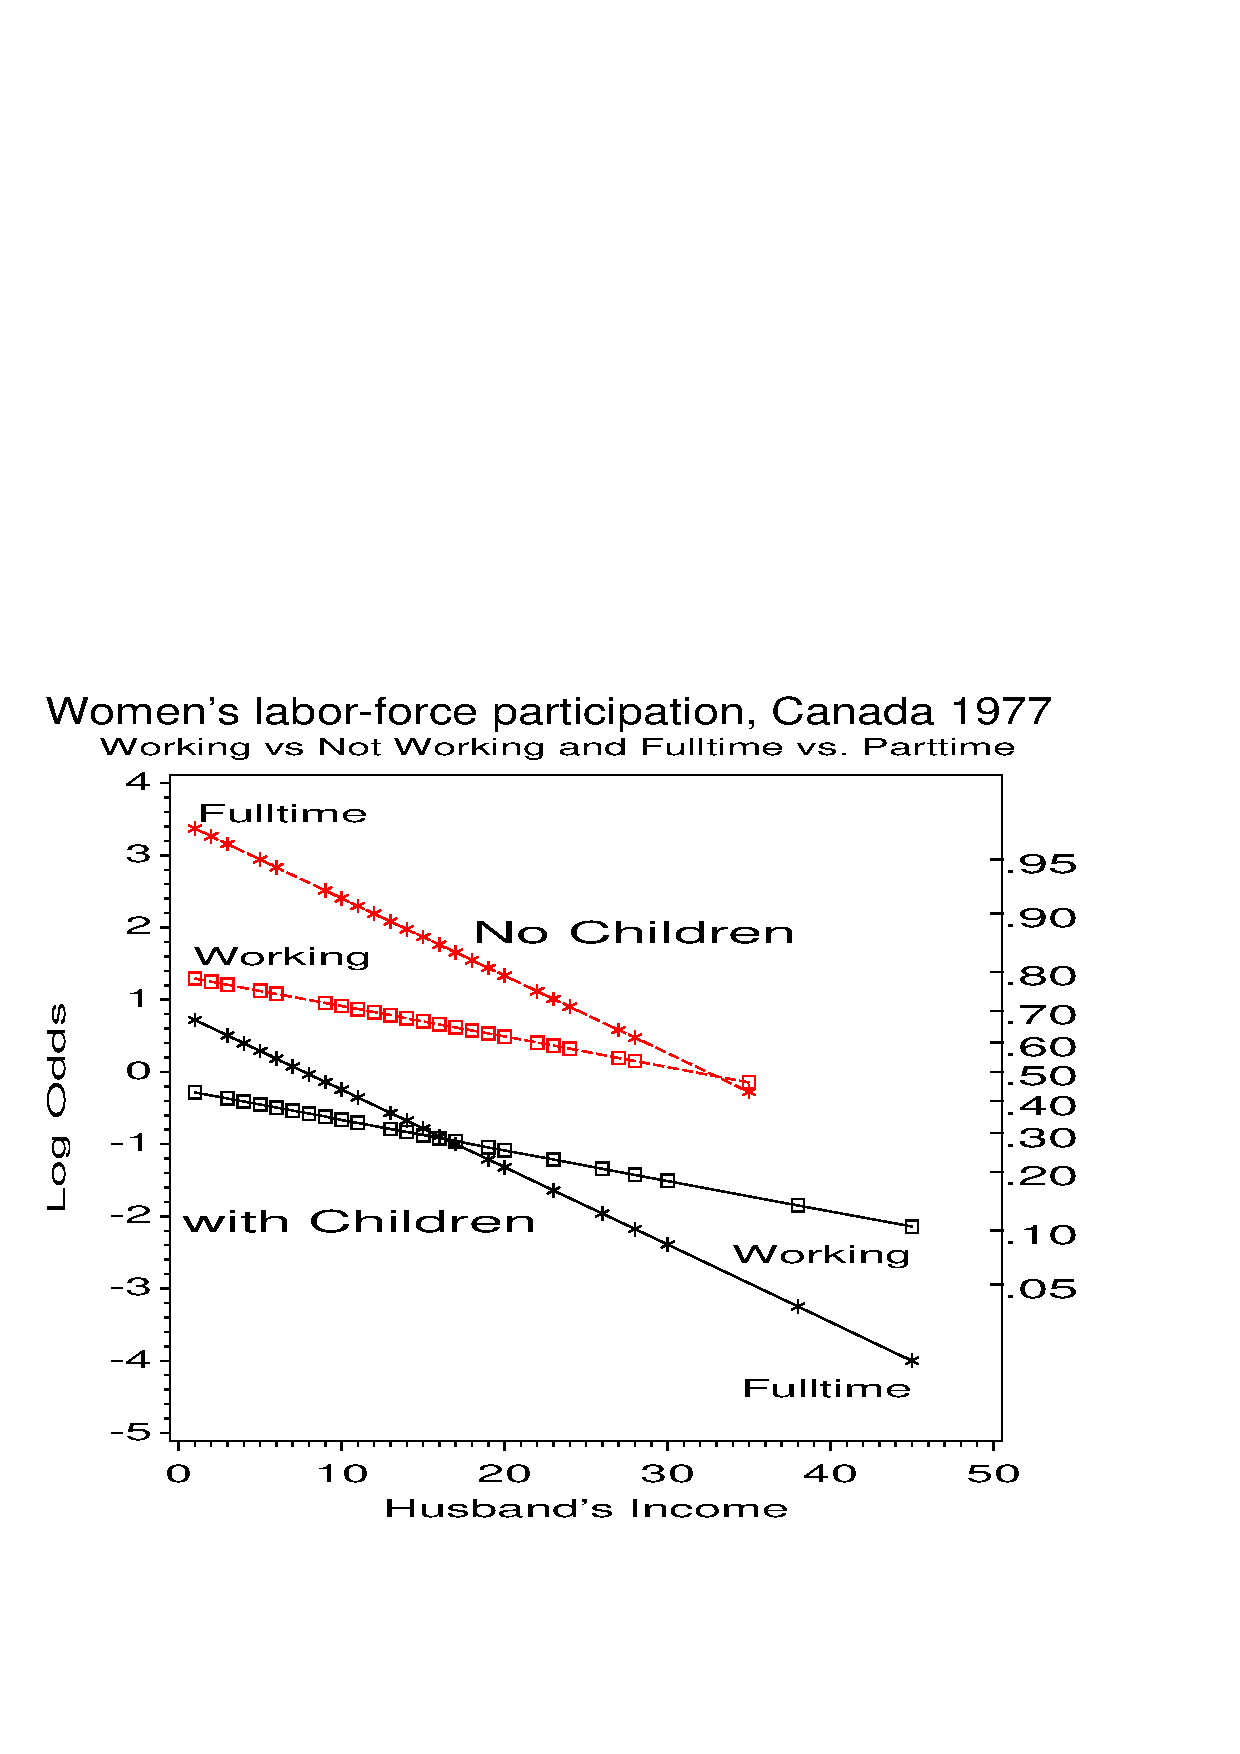
\includegraphics[height=.7\textheight]{fig/wlfpart}
\end{center}
\end{frame}

\begin{frame}[fragile]
  \frametitle{Model visualization}
  \begin{itemize*}
	\item Join \ODS{}s (\texttt{resultsw} and \texttt{resultsf})
	\item Combine Response \& Children $\rightarrow$ \texttt{event}
  \end{itemize*}
\begin{Input}
\sascomment{*-- Join the results datasets to create one plot;}
data both;
   set resultw(in=inw)     \sascomment{/* working  */}
       resultf(in=inf);    \sascomment{/* fulltime */}
   if inw then do;
      if children=1 then event='Working, with Children ';
      else event='Working, no Children ';
   end;
   else do;
      if children=1 then event='Fulltime, with Children ';
      else event='Fulltime, no Children ';
  end;
\end{Input}
\end{frame}

\begin{frame}[fragile]
  \frametitle{Model visualization}
\begin{comment}
  \begin{itemize*}
	\item \texttt{plot logit * husinc = event;} $\rightarrow$ separate lines
  \end{itemize*}
\end{comment}
\begin{Input}[baselinestretch=0.7]
proc gplot data=both;
   plot \sasemph{logit * husinc = event} /
        anno=lbl nolegend frame vaxis=axis1;
   axis1 label=(a=90 'Log Odds') order=(-5 to 4);
   title2 'Working vs Not Working and Fulltime vs. Parttime';
   symbol1 v=dot    h=1.5 i=join l=3 c=red;
   symbol2 v=dot    h=1.5 i=join l=1 c=black;
   symbol3 v=circle h=1.5 i=join l=3 c=red;
   symbol4 v=circle h=1.5 i=join l=1 c=black;
\end{Input}
\begin{center}
  \includegraphics[height=.55\textheight]{fig/wlfpart}
\end{center}
\end{frame}

\endinput

% slide template
\begin{frame}
  \frametitle{}
  \begin{itemize}
	\item{\large\bfseries }
      \begin{itemize*}
	  \item 
    	\begin{itemize*}
		\item 
		\item 
		\end{itemize*}
	  \item 
	  \end{itemize*}
	\item{\large\bfseries }
	\item{\large\bfseries }
  \end{itemize}
\end{frame}


\subsection{Generalized logit models}
\renewcommand{\FileName}{genlogit}
% slide template
\subsection{Basic ideas}
\begin{frame}
  \frametitle{Polytomous response: Generalized Logits}
  \begin{itemize}
	\item Models the probabilities of the $m$ response categories 
	as \(m - 1\) logits comparing
each of the first \(m - 1\) categories to the last (reference) category.
	\item Logits for any  pair of categories can be calculated
from the \(m - 1\) fitted ones.
	\item With $k$ predictors, \(x_1, x_2, \dots , x_k\), for $j=1, 2, \dots ,
	  m-1$, 
\begin{eqnarray*}
  L_{jm}  \equiv 
    \log \left( \frac{\pi_{ij}}{\pi_{im}} \right) & = & \beta_{0j}  +
  \beta _{1j} \,  x_{i1}  +
  \beta _{2j} \,  x_{i2}  + \cdots +
  \beta _{kj} \,  x_{ik} \quad \\
%  \mbox{for } j=1, 2, \dots , m-1 \\
  & = & \vec{\beta}_j \trans \vec{x}_i
\end{eqnarray*}

      \begin{itemize*}
	  \item One set of fitted coefficients, $\vec{\beta}_j$ for each
response category except the last.
	  \item Each coefficient, $\beta_{hj}$, gives the effect on the log odds
of a unit change in the predictor $x_h$
that an observation belongs to category $j$ vs.\ category $m$.
	  \end{itemize*}
	\item Probabilities in response caegories are calculated as:
\begin{equation*}
\pi_{ij} =
 \frac{ \exp ( \vec{\beta}_j \trans \vec{x}_i ) }
      { \sum_{j=1}^{m-1} \exp ( \vec{\beta}_j \trans \vec{x}_i ) }
	  \comma \, j=1,\dots, m-1 \,;
	  \quad\quad \pi_{im} = 1 - \sum_{j=1}^{m-1} \pi_{ij}
\end{equation*}
  \end{itemize}
\end{frame}

\begin{frame}[fragile]
  \frametitle{Polytomous response: Generalized Logits}
Fitting generalized logit models with SAS:
%  \begin{itemize}
%	\item SAS:
      \begin{itemize*}
	  \item Use \PROC{LOGISTIC} with \texttt{LINK=GLOGIT} option.
    	\begin{itemize*}
		\item \ODS\ $\rightarrow$ fitted probabilities, $\widehat{\pi}_{ij}$ for all $m$ categories
		\item Overall tests and specific tests for each predictor, for all $m$ categories
		\end{itemize*}
\vspace{2ex}
\begin{Input}[numbers=none]
proc logistic data=wlfpart;
   model labor = husinc children / \sasemph{link=glogit};
   output out=results p=predict xbeta=logit;
\end{Input}
	  \item Can also use \PROC{CATMOD} with \texttt{RESPONSE=LOGITS} statement.
    	\begin{itemize*}
		\item Same model, same predicted probabilities
		\item Different syntax, \ODS\ format, plotting steps
		\item Quantitative variables: \alert{\texttt{direct}} statement
		\end{itemize*}
\vspace{2ex}
\begin{Input}[numbers=none]
proc catmod data=wlfpart;
   \sasemph{direct husinc;}
   model labor = husinc children;
   \sasemph{response logits} / out=results;
\end{Input}
	  \end{itemize*} 

%  \end{itemize}
\end{frame}

\begin{frame}<1>[label=wlfpart5g]
  \frametitle{Example: Women's Labour Force Participation}
Graphs:
% two figures 
 \begin{minipage}[b]{.5\linewidth}
  \centering
  \includegraphics[width=.99\linewidth]{fig/wlfpart51}
 \end{minipage}%
 \begin{minipage}[b]{.5\linewidth}
  \centering
  \includegraphics[width=.99\linewidth]{fig/wlfpart52}
 \end{minipage}
\end{frame}


\begin{frame}[fragile]
  \frametitle{Example: Women's Labour Force Participation}
\begin{Input}[label=\fbox{\texttt{wlfpart5.sas} $\cdots$}]
title 'Generalized logit model';
proc logistic data=wlfpart;
   model labor = husinc children / \sasemph{link=glogit};
   \sasemph{output out=results p=predict xbeta=logit;}
\end{Input}
Response profile:
\begin{Output}[gobble=7]
                       Ordered                      Total
                         Value        labor     Frequency

                             1            1            66
                             2            2            42
                             3            3           155

             Logits modeled use labor=3 as the reference category.
\end{Output}
\emph{Note:} Not working is the baseline category
\end{frame}


\begin{frame}[fragile]
Overall and Type III tests:
\begin{Output}[gobble=7,baselinestretch=0.8]
                    Testing Global Null Hypothesis: BETA=0
 
            Test                 Chi-Square       DF     Pr > ChiSq

            Likelihood Ratio        77.6106        4         <.0001
            Score                   76.4850        4         <.0001
            Wald                    58.4351        4         <.0001

                          Type III Analysis of Effects
 
                                            Wald
                  Effect        DF    Chi-Square    Pr > ChiSq

                  husinc         2       12.8159        0.0016
                  children       2       53.9806        <.0001
\end{Output}
These are comparable to the combined tests for the nested dichotomies models.
\end{frame}

\begin{frame}[fragile]
Coefficients:
\begin{Output}[gobble=2,baselinestretch=0.8, fontsize=\footnotesize]
                    Analysis of Maximum Likelihood Estimates
 
                                          Standard          Wald
  Parameter    labor    DF    Estimate       Error    Chi-Square    Pr > ChiSq

  Intercept    1         1      1.9828      0.4842       16.7709        <.0001
  Intercept    2         1     -1.4323      0.5925        5.8445        0.0156
  husinc       1         1     -0.0972      0.0281       11.9762        0.0005
  husinc       2         1     0.00689      0.0235        0.0863        0.7689
  children     1         1     -2.5586      0.3622       49.9008        <.0001
  children     2         1      0.0215      0.4690        0.0021        0.9635
\end{Output}
i.e., the fitted models are:
\begin{eqnarray*}
  \log \left( \frac{ \Pr ( \mbox{fulltime} ) }
  { \Pr ( \mbox{not working} ) } \right) & = &
  1.983 - 0.097 \,  \mbox{H\$} - 2.56 \,  \mbox{kids} \\  %\label{eq:wlfgen1}
%
  \log \left( \frac{ \Pr ( \mbox{parttime} ) }
  { \Pr ( \mbox{not working} ) } \right) & = &
  -1.432 - 0.0069 \,  \mbox{H\$} - 0.0215 \,  \mbox{kids}  % \label{eq:wlfgen2}
\end{eqnarray*}
\emph{Interpretation:} Signs for \texttt{husinc} and \texttt{children} are understandable,
but need to make a plot!
\end{frame}

\begin{frame}[fragile]
\ODS\ \texttt{results} (for plots):
\begin{Output}[baselinestretch=0.7,gobble=2]
  case   labor   husinc  children   _LEVEL_     logit    predict

    1      3       15        1         1      -2.03423   0.09333
    1      3       15        1         2      -1.30743   0.19305
    1      3       15        1         3        .        0.71363
    2      3       13        1         1      -1.83977   0.11142
    2      3       13        1         2      -1.32122   0.18715
    2      3       13        1         3        .        0.70143
    3      3       45        1         1      -4.95114   0.00528
    3      3       45        1         2      -1.10067   0.24830
    3      3       45        1         3        .        0.74642
    4      3       23        1         1      -2.81207   0.04464
    4      3       23        1         2      -1.25230   0.21238
    4      3       23        1         3        .        0.74298
    5      3       19        1         1      -2.42315   0.06486
    5      3       19        1         2      -1.27987   0.20346
    5      3       19        1         3        .        0.73168
    6      3        7        1         1      -1.25639   0.18478
    6      3        7        1         2      -1.36257   0.16616
    ...
\end{Output}
\begin{itemize*}
	\item \texttt{logit} gives the two fitted log odds vs Not working
	\item \texttt{predict} gives the predicted probability for each category of \texttt{labor}
\end{itemize*}
\end{frame}

\begin{frame}[fragile]
  \frametitle{Example: Women's Labour Force Participation}
\begin{Input}[label=\fbox{$\cdots$ \texttt{wlfpart5.sas}},baselinestretch=0.7]
proc sort data=results;
   \sasemph{by children husinc _level_;}

   \sascomment{*-- Curve labels;}
%label(data=results, x=husinc, y=predict, cvar=_level_,
   by=children, subset=last._level_, text=put(_level_, labor.), 
   pos=2, out=labels1);

   \sascomment{*-- Panel labels;}
%label(data=results, x=20, y=0.85, 
   by=children, subset=last.children, text=put(children, kids.), 
   pos=2, size=2, out=labels2);
data labels;
   set labels1 labels2;
   by children;

goptions hby=0;
proc gplot data=results;
   \sasemph{plot predict * husinc = _level_} / 
      vaxis=axis1 hm=1 vm=1 \sasemph{anno=labels} nolegend;
   by children;
   axis1 order=(0 to .9 by .1) label=(a=90);
   symbol1 i=join v=circle   c=black;
   symbol2 i=join v=square   c=red;
   symbol3 i=join v=triangle c=blue;
   run;
\end{Input}
\end{frame}

\againframe<1>{wlfpart5g}
\endinput

% slide template
\begin{frame}
  \frametitle{}
  \begin{itemize}
	\item{\large\bfseries }
      \begin{itemize*}
	  \item 
    	\begin{itemize*}
		\item 
		\item 
		\end{itemize*}
	  \item 
	  \end{itemize*}
	\item{\large\bfseries }
	\item{\large\bfseries }
  \end{itemize}
\end{frame}


\section{Concluding remarks}
\section{Chapter summary}
\begin{itemize}
\item Discrete distributions typically involve basic \emph{counts} of occurrences
of some event occurring with varying frequencies.
\item The most commonly used discrete distributions include the binomial,
Poisson, negative binomial, geometric, and logarithmic series distributions.
Happily, these are all members of a family called the
power series distributions.
Methods of fitting an observed \Dset\ to any of these distributions are
described, and implemented in the \macro{GOODFIT}.
\item After fitting an observed distribution it is useful to plot the observed
and fitted frequencies.
Several ways of making these plots are described, and implemented in the
macro{ROOTGRAM}.
\item A graphical method for identifying which discrete distribution is most
appropriate for a given set of data involves plotting ratios
$k n_k / n_{k-1}$ against $k$.
These plots are constructed by the \macro{ORDPLOT}.
\item A more robust plot for a Poisson distribution involves plotting
a count metameter, $\phi ( n_k ) $ against $k$, which
gives a straight line (whose slope estimates the Poisson parameter)
when the data follows a Poisson distribution.
This plot provides robust confidence intervals for individual points
and provides a means to assess the influence of individual points
on the Poisson parameter.
These plots are provided by the \macro{POISPLOT}.
\item The ideas behind the Poissonness plot can be applied to the other
discrete distributions, as implemented in the \macro{DISTPLOT}.
\end{itemize}


\endinput
